\chapter{Measurement of $\xsecpsipptoDDbar$ near $\psipp$}
\label{ch:cross_section}

The main objective of this analysis is to measure the $\xsecpsipptoDDbar$ cross section at center-of-mass energies around the $\psipp$.
While the cross section very near the $\psipp$ mass has been measured with excellent precision \cite{ref:Toth:2014}, the shape over a wider energy range has not been measured as precisely.
As such, it has been impossible to fully determine the functional form that best describes the cross section or to definitively determine the extent which interference effects must be included.
Fits to this region with a single Breit-Wigner shape (i.e., no interference) have provided a unsatisfactory description of the $\psipp$.
The most straightforward modification of this assumption is to incorporate a contribution from the $\psip$.
This is the form considered here, where the procedure largely follows the methodology of the KEDR collaboration \cite{ref:Anashin:2012}.
With the larger statistics available at BESIII, however, an inclusive cross section measurement (such as performed by KEDR) is not required.
Instead, we measure the production of $\psipptoDD$ events directly.


\section{Derivation of $\xsecpsipptoDDbar$}
\label{sec:xsec_derivation}

The production rate for a pair of $D$ mesons coming from $\psipp$ at a given center-of-mass energy can be calculated following an approach of Kuraev and Fadin \cite{ref:Kuraev:1985}.
This method includes Initial State Radiation (ISR), which effectively replaces the well-defined $\ee$ center-of-mass energy of the accelerator with a distribution of energies, is given by the following:
\beq
\label{eq:xsec_rc}
\sigma^{RC}_{\DDbar}(W) = \int z_{\DDbar}(W \sqrt{1-x}) \, \sigma_{\DDbar}(W \sqrt{1-x}) \, \mathcal{F}(x, W^2) \, dx.
\eeq

\noindent 
Here, $W$ is the center-of-mass energy after the collision, $x$ parametrizes the fraction of radiated energy, and $\mathcal{F}(x, W^2)$ is the probability of losing this energy by ISR:
\label{eq:fancy_f}
\begin{align}
\mathcal{F}(x, W^2) &= \beta \, x^{\beta - 1} \left[ 1 + \frac{\alpha}{\pi} \left( \frac{\pi^2}{3} - \frac{1}{2} \right) + \frac{3}{4} \beta + \beta^2 \left( \frac{37}{96} - \frac{\pi^2}{12} - \frac{L}{72} \right) \right] = \beta \, x^{\beta - 1} F(W^2), \notag \\ 
& \qquad \qquad \qquad \beta = \frac{2 \alpha}{\pi} (L - 1), \qquad L = \log \left( \frac{W^2}{m_e^2} \right).
\end{align}

\noindent
The factor $z_{\DDbar}$ accounts for the expected Coulomb interaction between the mesons for the charged mode ($\Dp \Dm$),
\beq
\label{eq:z_Dp}
z_{\Dp \Dm} = \frac{\pi \alpha / \beta_{\Dp} }{ 1 - \text{exp} (-\pi \alpha / \beta_{\Dp} ) } \times \theta (W - 2 m_{\Dp} ),
\eeq

\noindent 
but only accounts for the $\DDbar$ energy threshold in the neutral mode ($\DO \aDO$),
\beq
\label{eq:z_D0}
z_{\DO \aDO} = \theta (W - 2 m_{\DO} ).
\eeq

\noindent
The theta function imposes the step in the cross section at the production threshold.
 
The integral in Eq. \ref{eq:xsec_rc} can be simplified by taking advantage of the relatively constant values of $z_{\DDbar}$ and $\sigma_{\DDbar}$ over sufficiently small intervals.
By splitting the full $W$ range into such intervals approximating the integral over each, this becomes
\beq
\int \mathcal{F}(x, W^2)~dx \approx \sum\limits_{n=0}^N F(W^2) \int_{\tfrac{n}{N}}^{\tfrac{n+1}{N}} \beta x^{\beta-1}~dx = \sum\limits_n^N F(W^2) \left[ x_{\text{upper}}^\beta - x_{\text{lower}}^\beta \right].
\eeq

\noindent 
The upper, lower, and mid-point values are given by
\beq
\renewcommand\arraystretch{1.0}
\label{eq:x_terms}
x_i = \left[ 1 - \left( \frac{ 2 m_D}{ W } \right)^2 \right] \left( \frac{n_i}{ N } \right),
\qquad n_i : 
\begin{cases}
    n_{\text{lower}} &= n \\[-0.7em]
    n_{\text{mid}}   &= n + \tfrac{1}{2} \\[-0.7em]
    n_{\text{upper}} &= n + 1 
\end{cases}.
\eeq

\noindent
The bracketed expression in Eq. \ref{eq:x_terms} represents the maximum value of $x$ determined by the theta functions of Eqs. \ref{eq:z_Dp} and \ref{eq:z_D0}.
To maintain sufficient precision with this interval approximation, the value of $N = 1024$ is used.
Combining this with the other factors in Eq. \ref{eq:xsec_rc}, the cross section including the effect of ISR becomes
\beq
\label{eq:xsec_rc_simp}
\sigma^{RC}_{\DDbar}(W) = \sum_{n = 0}^N z_{\DDbar}(W') \, \sigma_{\DDbar}(W') \, F(W^2) \left[ 1 - \left( \frac{ 2 m_D}{ W } \right)^2 \right]^\beta \left[ \frac{ [(n + 1)^\beta - n^\beta] }{ N^\beta } \right],
\eeq
where $W' = W \sqrt{1 - x_{\text{mid}}}$.
The Born level (lowest order) $\DDbar$ cross section is given by
\beq
\label{eq:born_xsec}
\sigma_{\DDbar} = \frac{ \pi \alpha^2 }{ 3 W^2 } \beta_D^3 |F_D(W)|^2, \qquad \beta_D = \sqrt{1 - \frac{ 4 m_D^2 }{ W^2 } }.
\eeq

\noindent
Here, $\beta_D$ is the velocity of the $D$ meson in the center-of-mass system.
The form factor $F_D$ governs the contributions of each individual resonant ($R$) component and the total non-resonant ($NR$) component.
Each resonant piece is parametrized with a phase angle relative to the non-resonant contribution:
\beq
\label{eq:form_factor}
F_D(W) = F_D^{\text{NR}}(W) + \sum_r F^{R_r}_D(W) \, e^{i \phi_r }.
\eeq

\noindent
Each resonant contribution to the form factor is modeled by a Breit-Wigner amplitude,
\beq
\label{eq:breit_wigner}
F^R_D(W) = \frac{ 6 \, W \sqrt{ (\Gamma_{ee} / \alpha^2 ) ( \Gamma_{\DDbar}(W) / \beta^3_D ) } }{ M^2 - W^2 - i M \Gamma(W) },
\eeq

\noindent 
where $\Gamma_{ee}$ is the dielectron partial width, and $\Gamma(W)$ represents the total width of the resonance with mass $M$: 
\beq\label{eq:Gamma}
\Gamma(W) = \left( \frac{M}{W} \right) \left[ \frac{ z_{\DDbar}(W) \, d_{\DDbar}(W) }{ z_{\DO \aDO}(M) \, d_{\DO \aDO}(M) + z_{\Dp \Dm}(M) \, d_{\Dp \Dm}(M) } \right] \Gamma(M).
\eeq

\noindent
The value of $\Gamma(M)$ represents the total width at the nominal mass of the resonance, while $d_{\Dp \Dm}$ and $d_{\DO \aDO}$ are the Blatt-Weisskopf damping factors \cite{ref:Blatt:1952} for a vector resonance:
\beq
\label{eq:blatt_weisskopf}
d_{\DDbar} = \frac{ \rho_{\DDbar}^3 }{ \rho_{\DDbar}^2 + 1 }, \qquad \rho_{\DDbar} = q_D R_0 = \left( \frac{ \beta_D \, W }{ 2 } \right) R_0.
\eeq

\noindent
Here, $q_D$ is the $D$ momentum in the center-of-mass frame, while $R_0$ represents the radius of the parent particle. 
The $\DDbar$ partial width listed in Eq. \ref{eq:breit_wigner} is the total width rescaled according to $\BnDD$, the sum of all non-$\DDbar$ decay modes of $\psipp$:
\beq
\label{eq:Gamma_DDbar}
\Gamma_{\DDbar}(W) = \Gamma(W) \times (1 - \BnDD).
\eeq
Theoretical calculations of $\BnDD$ place the value on the order of a few percent.
However, experimental results have measured values throughout the range of \SIrange{0}{16}{\%}.
Without a trustworthy measurement to use for our analysis, we elect to define the fit parameter $\Geepsipp$ to include the product with (1 - $\BnDD$).
While this does not provide an immediate result, future values for either parameter allows the other to be easily determined.
More information about the branching fraction is discussed in \Cref{ch:non_DDbar}.


\section{Form Factors}
\label{sec:form_factors}
To apply the cross section formula derived above, the relevant form factors (\Cref{eq:form_factor}) must now be specified.
We assume the $\psip$ resonant contribution is negligible in the energy range of our measurements, so the only significant resonant contribution is from the $\psipp$:
\beq
F_D(W) = F_D^{\text{NR}}(W) + F^{\psipp}_D(W) \, e^{i \phi^{\psipp} }.
\eeq

\noindent
Currently, there is no definitive model for the non-resonant term, so we use two alternative parameterizations.
The first is a simple exponential model:
\beq
\label{eq:exp_model}
F_D^{NR} = \FNR \, \exp ( -q_D^2 / \aNR^2 ),
\eeq

\noindent 
where both $\FNR$ and $\aNR$ are left free in the fit to the cross section.
The second treatment implements a Vector Dominance Model (VDM).
This assumes the interference effects are due to the $\psip$ mediating $\DDbar$ production above threshold,
\beq
\label{eq:vdm_model}
F_D^{NR}(W) = F_D^{\psip}(W) + F_0,
\eeq

\noindent
and that the effective properties of the $\psip$ are similar to those of the $\psipp$.
The real constant $F_0$ represents the potential effect of higher resonances, like the $\psi(4040)$.
The first term is similar to \Cref{eq:breit_wigner}, but with a modification to the total width,
\beq
\label{eq:Gamma_psip}
\Gpsip(W) = \left( \frac{M^{\psip}}{W} \right) \left[ \frac{ zd_{\DO \aDO}(W) + zd_{\Dp \Dm}(W) }{ zd_{\DO \aDO}(M^{\psi''}) + zd_{\Dp \Dm}(M^{\psi''}) } \right] \Gpsip(M),
\eeq

\noindent
where $zd_{\DDbar}(W) = z_{\DDbar}(W) \times d_{\DDbar}(W)$.
Without this modification, the mass of the $\psip$ would be below the $\DDbar$ threshold, and thus, the vanishing $z_{\DDbar}$ terms would cause a singularity in the width.
Therefore, we use the mass of the $\psipp$ in its place to estimate the effects in this region.
While it may behave like the total width in \Cref{eq:Gamma_psip}, the true the physical meaning of the parameter $\Gpsip(W)$ is unclear.

For the radii in \Cref{eq:blatt_weisskopf}, however, the values used are distinct for each meson: $R_{\psip} = \SI{0.75}{\fm}$ and $R_{\psipp} = \SI{1.00}{\fm}$.
These are the same values as used in the KEDR procedure \cite{ref:Anashin:2012}, where each is quoted with an uncertainty of 25\%.
This provides one of the largest sources of systematic uncertainty, and is discussed in \Cref{sec:systematics}.


\section{Data and Monte Carlo Samples}
\label{sec:samples}

\subsection{Data Samples}
\label{ssec:data_samples}

This analysis primarily uses scan data produced by BEPCII and collected by BESIII in 2010 over an energy range of \SIrange{3.643}{3.890}{\GeV}.
These data are partitioned into 34 center-of-mass energy ($\Ecm$) bins of variable size over a range of \SIrange{3.735}{3.870}{\GeV}.
The bin partitioning was determined from measurements of center-of-mass energies (\Cref{ssec:energy_measurement}).
The total range was chosen to be above the $\DO\aDO$ threshold (\SI{3.730}{\GeV}) and below the $D^{*0}\aDO$ threshold (\SI{3.872}{\GeV}).
Note, this includes values below the $\Dp \Dm$ threshold (\SI{3.739}{\GeV}), with production beginning in the third bin.

Additionally, there are three higher statistics points used for comparison.
These include an `On-Peak $\psipp$' sample of \SI{2.93}{\invfb} at $\Ecm = \SI{3.7732}{\GeV}$, an `$XYZ$-scan' sample of \SI{50.54}{\invpb} at $\Ecm = \SI{3.810}{\GeV}$, and an `$R$-scan' sample of \SI{7.95}{\invpb} at $\Ecm = \SI{3.850}{\GeV}$.
The first of these is the high statistics measurement very near the $\psipp$ peak that was used for a double-tag reconstruction (both $\D$ and $\aD$ reconstructed in a single event) measurement performed by Derrick Toth \cite{ref:Toth:2014}.
The other two samples were analyzed using the same procedure as for the scan data (See \Cref{sec:signal,sec:efficiency,sec:fitting}).
None of these points are used to determine the final results, as the differences between samples introduce additional systematics which degrade any statistical improvement.
However, these provide useful comparisons of cross section measurements at important energy points for the primary scan sample.


\subsection{Center-of-Mass Energy Measurement}
\label{ssec:energy_measurement}

To precisely determine the values of center-of-mass energy along the scan data region, $\ee \rightarrow \mumu$ events were analyzed to determine their invariant mass ($\minv$).
Assuming that minimal energy is radiated by the muons, this value is effectively equal to the energy produced by the collider.
The selection process for such events is shown in \Cref{tab:muon_cuts}.
The statistics of the scan data are too small to precisely determine the energy for individual runs.
Therefore, multiple runs were combined together into bins based on the assumption that run groups were taken at nearly identical energies.
A comparison of the measured values to the less well calibrated beam energies measured by BEPCII during runtime is shown in \Cref{fig:scan_E_cm_fit}.

\begin{table}[H]
\centering
\renewcommand\arraystretch{1.0}
\begin{tabular}{c| c}%D{<}{\; < \;}{-1} }
\hline
Vertex ($xy$) & $V_{xy} < \pp \SI{1}{\cm}$ \\
Vertex ($z$)  & $|Vz|   < \SI{10}{\cm}$ \\
MDC Angle          & $|\cos\theta|^{\mu^\pm} < 0.80$ \\
Muon Opening Angle & $\cos(179.64^\circ) < \cos\theta_{\mu\mu} < \cos(178.60^\circ)$ \\
Energy-Momentum Ratio & $0.05 \leq (E / p)^{\mu^\pm} < 0.15$ \\ 
Shower Energy & $\SI{0.0}{\GeV} < E_{EMC}^{\mu^\pm} < \SI{0.3}{GeV}$ \\
\hline
\end{tabular}
\caption{Selection cuts on muon tracks used to determine the center-of-mass energy.}
\label{tab:muon_cuts}
\end{table}

\begin{figure}[H]
\centering
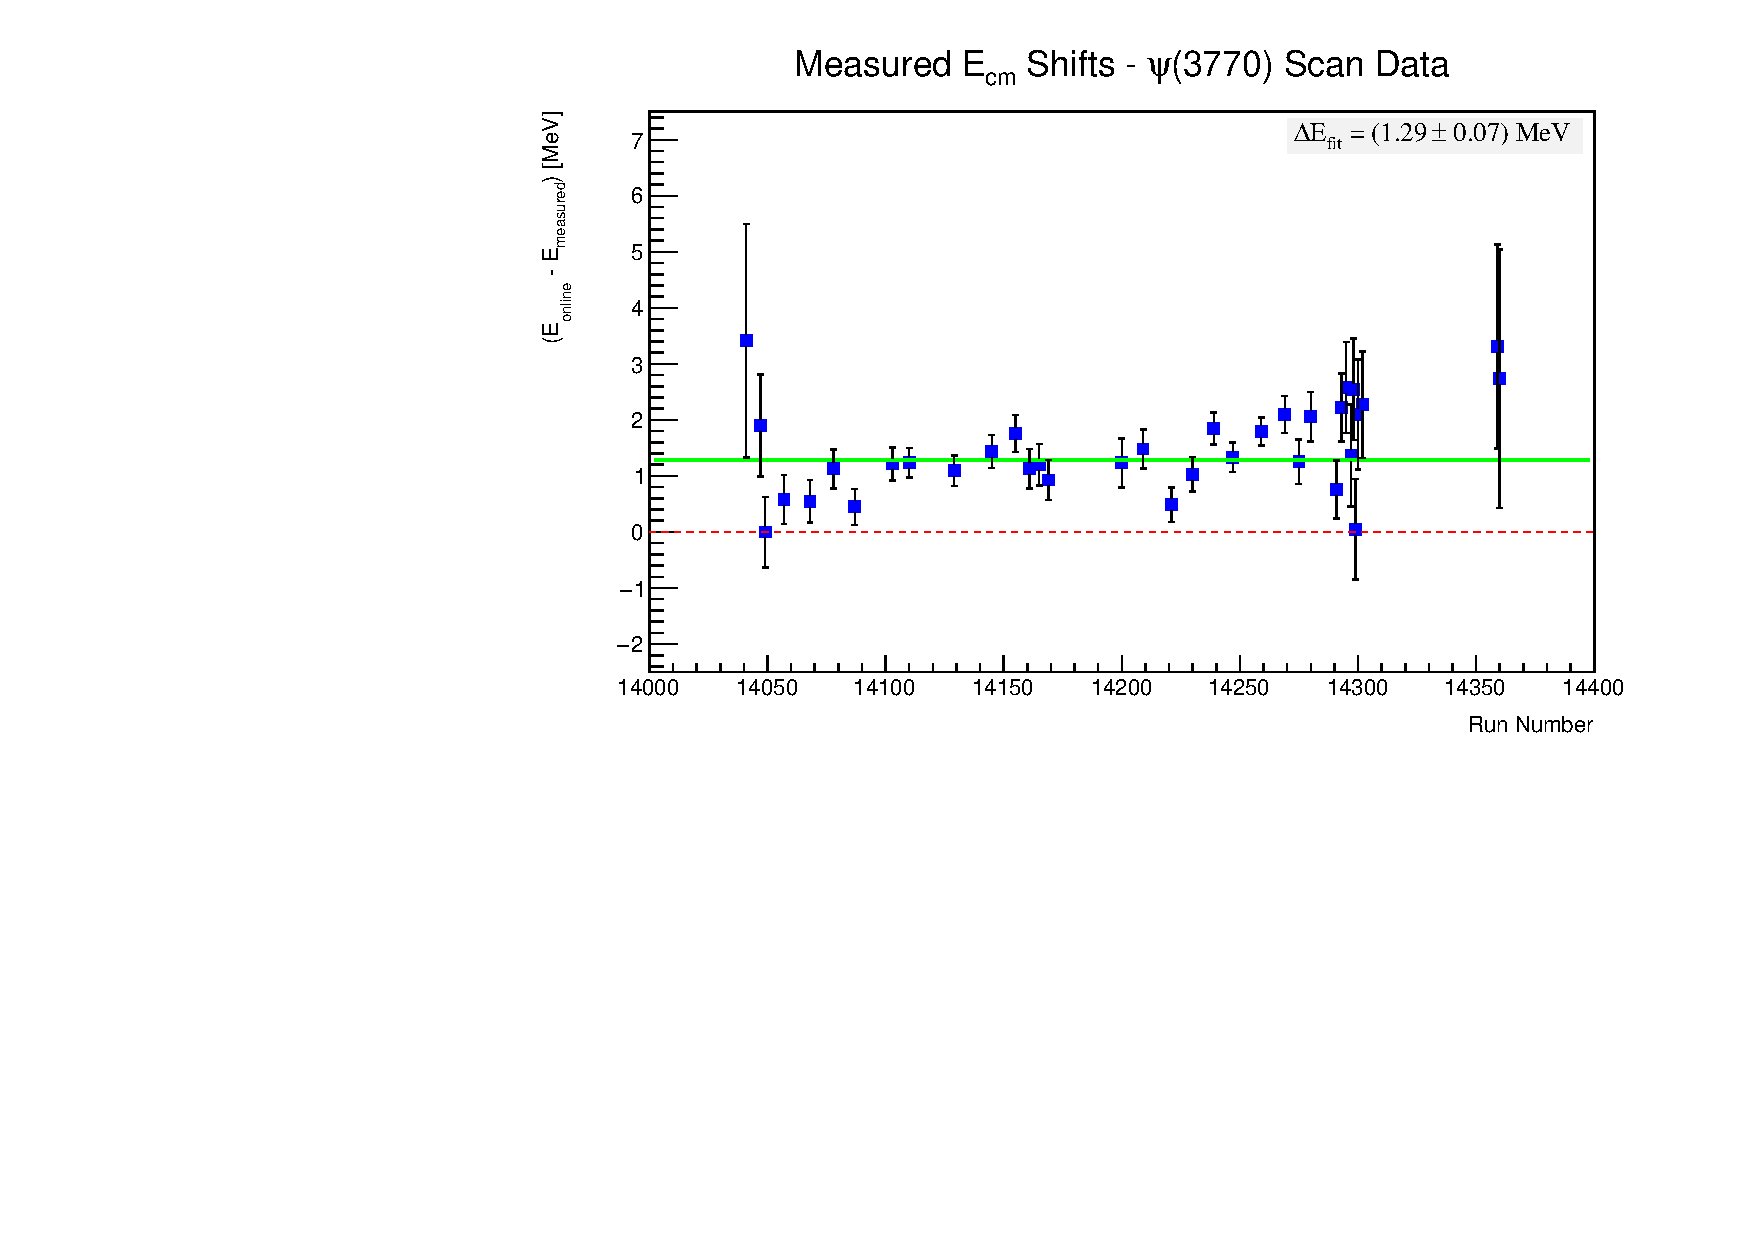
\includegraphics[scale=0.75]{figures/plots/E_cm_shifts_scan_fit_cut_new.pdf}
\caption{A comparison of online center-of-mass energies and measured $\mumu$ events.}
{The average value of the $\mumu$ pair measurements (green) is higher than the average value of the online BEPCII measurements (red) by about \SI{1.29}{\MeV}.}
\label{fig:scan_E_cm_fit}
\end{figure}


The use of muons to determine energy is subject to an overall scale shift due to potentially miscalibrated momentum measurements, most likely due to the magnetic field.
This requires a point of reference to ensure that the measured values are correctly determined.
We use the first round of the on-peak $\psipp$ sample for this comparison, as its center-of-mass energy has been measured very precisely using an independent technique involving $\DDbar$ events \cite{ref:Dong:2014}.
The results of this method compared to our own are shown in \Cref{fig:on_peak_E_cm_fit}.
It is evident the procedure using $\DDbar$ events provides more stability over the run range than using dimuon events.

\begin{figure}[H]
\centering
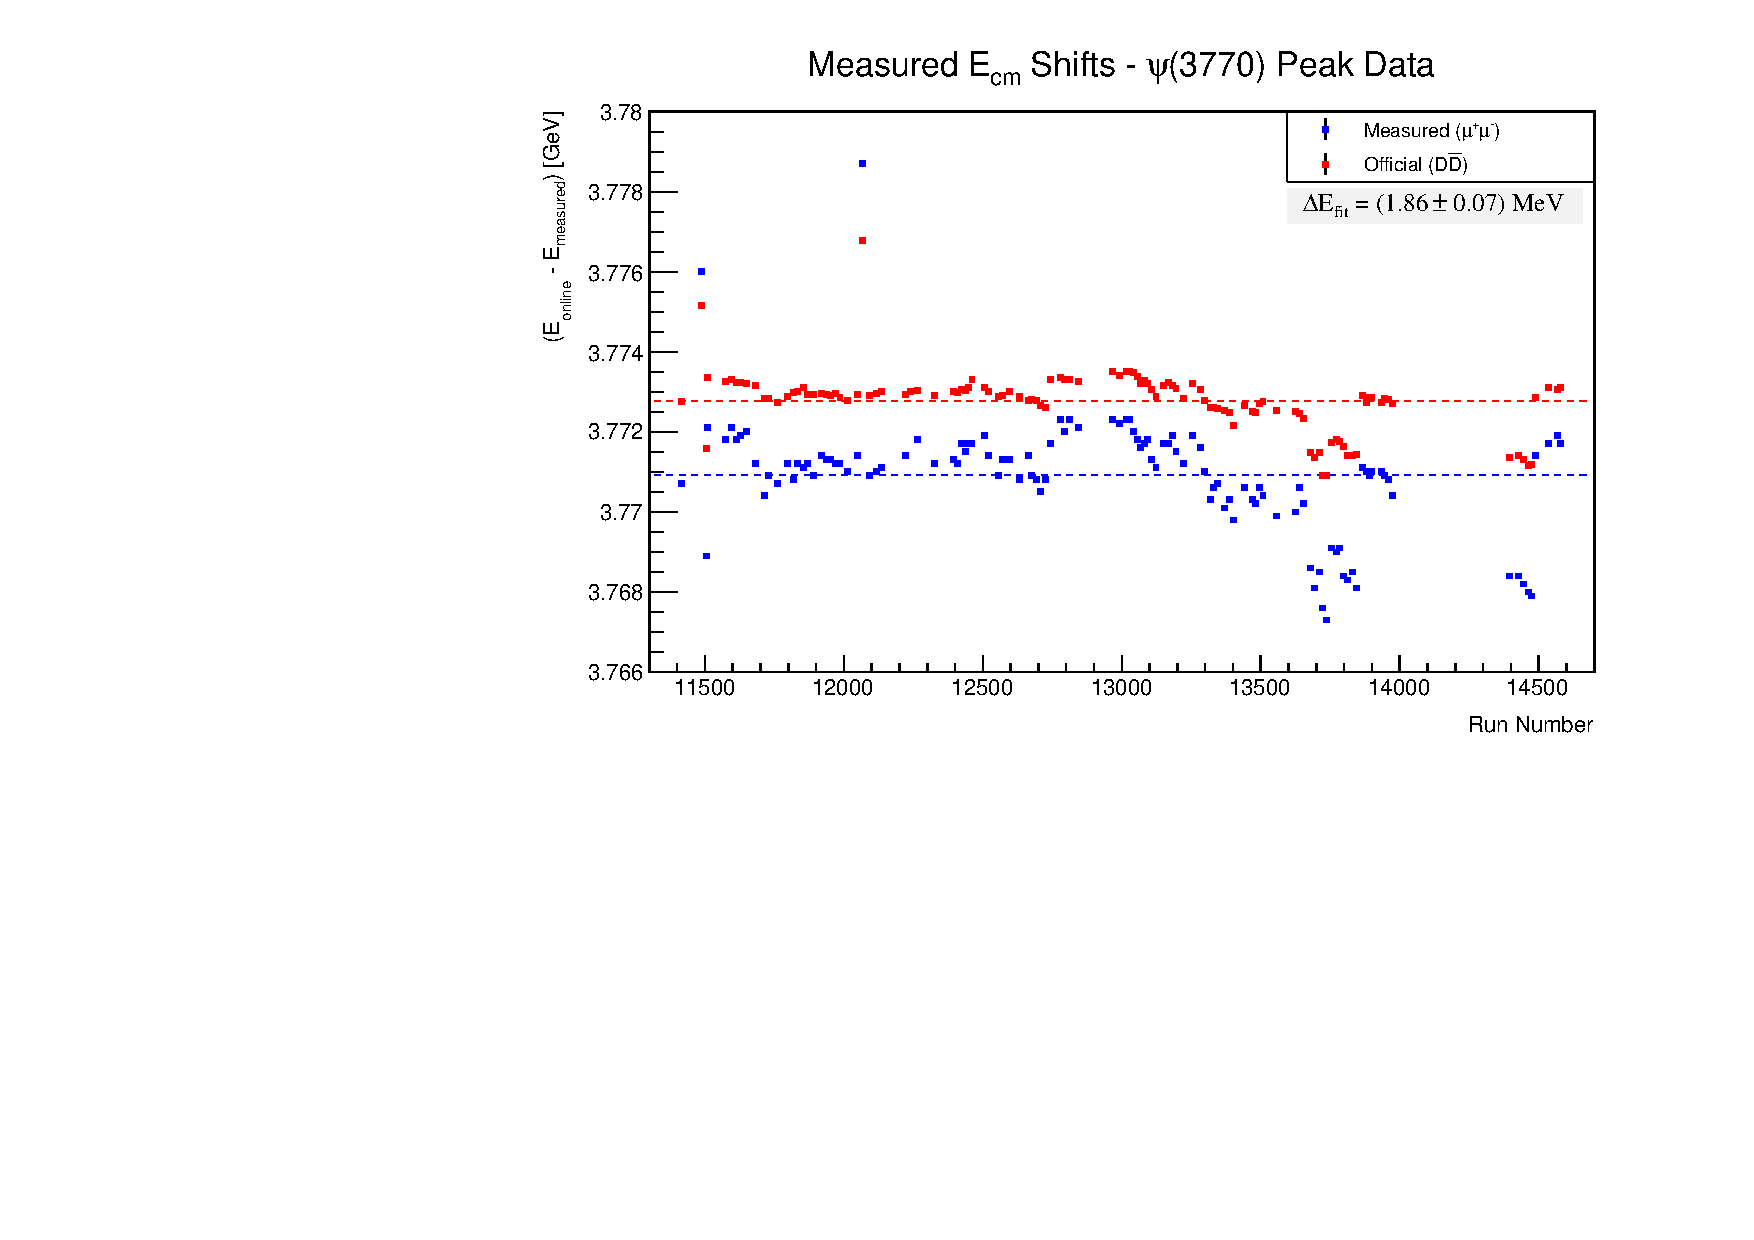
\includegraphics[scale=0.75]{figures/plots/E_cm_fit_cut_new.pdf}
\caption{The values measured for on-peak data center-of-mass energies.}
{The difference between our measured values (blue) and the official values (red) is used to shift the results of the measured scan data energy values.}
\label{fig:on_peak_E_cm_fit}
\end{figure}

To correct our measurements for the scan data, we use the difference in average values between the two methods, $\DeltaE_{\DDbar} - \DeltaE_{\mumu} \approx \SI{1.86}{\MeV}$ (see \Cref{fig:scan_E_cm_fit}). 
Adding this difference to each scan data measurements, we obtain the center-of-mass values used in this analysis.
Comparing this to the initial scan data center-of-mass energies, which were higher than the measured values by \SI{1.29}{\MeV} (see \Cref{fig:on_peak_E_cm_fit}), we find the initial values of the scan data were notably low ($\SI{1.86}{\MeV} - \SI{1.29}{\MeV} \approx \SI{0.7}{\MeV}$).
In regions where the cross section rapidly changes, this can have a dramatic effect on determining the functional shape.
Namely, this would correspond to a measured mass for the $\psipp$ which is off by \SI{0.7}{\MeV}.
% From this procedure, we find the initial values of scan data energy were lower than these measured values by \SI{1.86}{\MeV} - \SI{1.29}{\MeV} $\approx$ \SI{0.7}{\MeV} on average, where the values are taken from \Cref{fig:scan_E_cm_fit,fig:on_peak_E_cm_fit}.
The final center-of-mass energies of the scan data, along with the luminosity of each bin, are shown in \Cref{tab:luminosity}.

\pagebreak

\subsection{Luminosity Measurement}
\label{ssec:luminosity_measurement}

To precisely determine the values of integrated luminosity for each bin, radiative Bhabha events ($\bhabha (\gamma)$) were analyzed following the procedure of Ref. \cite{ref:Hafner:2015}.
For each run, \num{1.4e6} simulated events were generated using Babayaga 3.5 to characterize the detector response.
We select events with only two (oppositely) charged tracks, satisfying the criteria shown in \Cref{tab:bhabha_cuts}.

\begin{table}[H]
\centering
\renewcommand\arraystretch{1.0}
\begin{tabular}{c| D{<}{\; < \;}{-1} }
\hline
Vertex ($xy$) & V_{xy} < \pp \SI{1}{\cm} \\
Vertex ($z$)  & |Vz|   < \SI{10}{\cm} \\
MDC Angle         & |\cos\theta| < 0.80 \\
Exclude $\ee \rightarrow \mu^+ \mu^- (\gamma)$ Events & \multicolumn{1}{c}{ $E_{\text{EMC}} > 0.73 \times \Ebeam$ } \\
Exclude $\ee \rightarrow \gamma \jpsi, \; \jpsi \rightarrow \ee$ Events & \multicolumn{1}{c}{$p > 0.93 \times \Ebeam$ } \\
\hline
\end{tabular}
\caption{Selection cuts on electron tracks used to determine the luminosity.}
\label{tab:bhabha_cuts}
\end{table}

Applying these cuts to both data and MC identically, we use the resulting number of events found in the MC divided by the number of total generated events to determine the efficiency $(\epsilon_{MC})$.
From this, and using the cross section provided by the generator $(\sigma_{\text{Bhabha}})$, we can determine the integrated luminosity $(\lum)$ of each run from the number of events passing the same cuts in data $(N_{\text{data}})$:
\beq
\lum = \frac{N_{\text{data}}}{\sigma_{\text{Bhabha}} ~ \epsilon_{MC}}
\eeq
The integrated luminosity for each bin is shown in \Cref{tab:luminosity}.
The total luminosity for the scan data used is $(69.80 \pm 0.03 \pm 0.70)$ \si{\invpb}, where the errors are statistical and systematic, respectively.
Effects from the systematic error are examined in \Cref{sec:systematics}.

\begin{table}[H]
\centering
\renewcommand\arraystretch{1.0}
\begin{tabular}{r l c l}
\hline
Bin & Run Range & $\Ecm$ Range [\si{\GeV}] & $\lum$ [\si{\invpb}] \\
\hline
 0 & 14041 - 14046 & 3.734 - 3.736 & 0.8293(30) \\
 1 & 14360 - 14360 & 3.736 - 3.744 & 0.3287(19) \\
 2 & 14047 - 14048 & 3.744 - 3.748 & 0.9524(32) \\
 3 & 14049 - 14053 & 3.748 - 3.750 & 1.4055(39) \\
 4 & 14057 - 14067 & 3.750 - 3.751 & 2.2717(50) \\
 5 & 14068 - 14077 & 3.751 - 3.753 & 2.9702(57) \\
 6 & 14078 - 14086 & 3.753 - 3.755 & 3.3080(60) \\
 7 & 14087 - 14101 & 3.755 - 3.756 & 3.4162(61) \\
 8 & 14103 - 14109 & 3.756 - 3.759 & 3.8712(65) \\
 9 & 14110 - 14123 & 3.759 - 3.762 & 4.4382(70) \\
10 & 14129 - 14144 & 3.762 - 3.765 & 4.4896(70) \\
11 & 14145 - 14154 & 3.765 - 3.767 & 3.2828(60) \\
12 & 14155 - 14160 & 3.767 - 3.771 & 2.4418(52) \\
13 & 14161 - 14164 & 3.771 - 3.774 & 2.0151(47) \\
14 & 14165 - 14168 & 3.774 - 3.777 & 1.8261(45) \\
15 & 14169 - 14174 & 3.777 - 3.780 & 1.8237(45) \\
16 & 14200 - 14203 & 3.780 - 3.782 & 1.9505(46) \\
17 & 14209 - 14217 & 3.782 - 3.787 & 2.1500(49) \\
18 & 14221 - 14226 & 3.787 - 3.789 & 2.5488(53) \\
19 & 14230 - 14238 & 3.789 - 3.792 & 2.8320(56) \\
20 & 14239 - 14246 & 3.792 - 3.797 & 3.5310(63) \\
21 & 14247 - 14258 & 3.797 - 3.800 & 4.0479(67) \\
22 & 14259 - 14268 & 3.800 - 3.802 & 3.9284(66) \\
23 & 14269 - 14274 & 3.802 - 3.807 & 2.6929(55) \\
24 & 14275 - 14279 & 3.807 - 3.809 & 1.7604(44) \\
25 & 14280 - 14290 & 3.809 - 3.813 & 1.2539(38) \\
26 & 14291 - 14292 & 3.813 - 3.815 & 0.8969(32) \\
27 & 14293 - 14294 & 3.815 - 3.823 & 0.6803(28) \\
28 & 14295 - 14296 & 3.823 - 3.832 & 0.3997(21) \\
29 & 14297 - 14297 & 3.832 - 3.839 & 0.2846(18) \\
30 & 14298 - 14298 & 3.839 - 3.849 & 0.2802(18) \\
31 & 14299 - 14299 & 3.849 - 3.855 & 0.2764(18) \\
32 & 14300 - 14301 & 3.855 - 3.863 & 0.3188(19) \\
33 & 14302 - 14303 & 3.863 - 3.870 & 0.3002(19) \\
\hline
\end{tabular}
\caption{Measured integrated luminosities for each energy bin.}{The uncertainties listed are statistical errors from the data selection, as uncertainties from the MC statistics are negligible.}
\label{tab:luminosity}
\end{table}


\subsection{Monte Carlo Generation}
\label{ssec:monte_carlo}

To analyze the detection efficiencies and background levels of the detector, several MC samples were produced.
For the signal determination, samples of generic $\DO \aDO$ and $\Dp \Dm$ from $\psipp$ were generated with \num{2e5} events per center-of-mass energy bin.
In addition, $100\times$ data-size samples were produced for $\qqbar$, $\tautau$, radiative return to $\jpsi$ (denoted $\gamma \jpsi$), and radiative return to $\psip$ (denoted $\gamma \psi'$).
Each of these samples was generated at the University of Minnesota in July of 2014 using BOSS version 6.6.4.p02.
The $\DO \aDO$, $\Dp \Dm$, $\qqbar$, and $\tautau$ states were generated using KKMC, while the $\gamma \jpsi$ and $\gamma \psi'$ were generated with BesEvtGen.
All except $\qqbar$ were then decayed with BesEvtGen.
The total numbers of events in each sample is shown in \Cref{tab:mc_samples}.

\begin{table}[H]
\centering
\renewcommand\arraystretch{1.0}
\begin{tabular}{c c}
\hline
Sample & Number of Events \\
\hline
$\psipp \rightarrow \DO \aDO$ & \num{6.800e6} \\
$\psipp \rightarrow \Dp \Dm$  & \num{6.400e6} \\
$\qqbar$                      & \num{8.916e7} \\
$\gamma \jpsi$                & \num{7.307e6} \\
$\gamma \psi'$                & \num{2.457e7} \\
$\tautau$                     & \num{2.164e7} \\
% Data                          & \num{4.844e8} \\
\hline
\end{tabular}
\caption{Number of events contained in each generated sample.}% and the scan data.}
\label{tab:mc_samples}
\end{table}

In general, all MC samples were generated based on decay tables developed and maintained within BESIII based on world-average branching fraction measurements. 
The $\DDbar$ samples were generated by implementing the Born level shape measured in this analysis into KKMC.
This procedure was iterated five times to provide a data-driven basis for the ISR corrections.
The effects of this process are examined in \Cref{sec:systematics}.


% \subsection{Software Packages}
% \label{ssec:software}
% 
% The main BESIII software packages used for this analysis are shown in \Cref{tab:software_packages}.
% The package \texttt{DTagRecAlg} is a custom package used to extract variables relevant to this analysis from the default BESIII version of \texttt{DTagAlg}.
% 
% \begin{table}[H]
% \centering
% \renewcommand\arraystretch{1.0}
% \begin{tabular}{c c}
% \hline
% Package & Version \\
% \hline
%     KKMC       & v00-00-51 \\
%     DTagAlg    & v00-00-51 \\
%     DTagRecAlg & v00-00-01 \\
% \hline
% \end{tabular}
% \caption{The software packages used in this analysis and their version numbers.}
% \label{tab:software_packages}
% \end{table}

\pagebreak


\section{Signal Determination}
\label{sec:signal}

We measure the yields of both $\DO \aDO$ and $\Dp \Dm$ events with two-dimensional fits to $\DeltaE$ and $\mbc$, as defined in \ref{ssec:dtag_reconstruction}.
MC samples are partitioned into the following four groups: proper $D$-tags ($N_{\DDbar}$), misreconstructed $D$-tags ($N_{\text{misrec}}$), continuum ($N_{\qqbar}$), and other ($N_\text{other}$).
The first two groups are obtained using truth information from the $\DDbar$ samples, while the last group is a combination of the $\tautau$, $\gamma \jpsi$, and $\gamma \psi'$ samples.
These groups are fitted to data using the RooFit \cite{ref:RooFit} package to perform a negative log-likelihood minimization for each energy bin ($E_i$) separately for both $\DO$ and $\Dp$.
For each fit, the four MC sample groups are used to construct 2D ($\DeltaE$ vs. $\mbc$) PDF functions that are used to fit the corresponding data histograms.
The proper $\DDbar$ shape is treated as signal, and its integral after fitting $(N_{D})$ is used for determining the signal yields and cross sections.
An example fit is shown in \Cref{fig:example_fit}, while the complete set of these plots can be found in \Cref{app:D0_signal_fits,app:Dp_signal_fits}.

\begin{figure}[h]
\centering
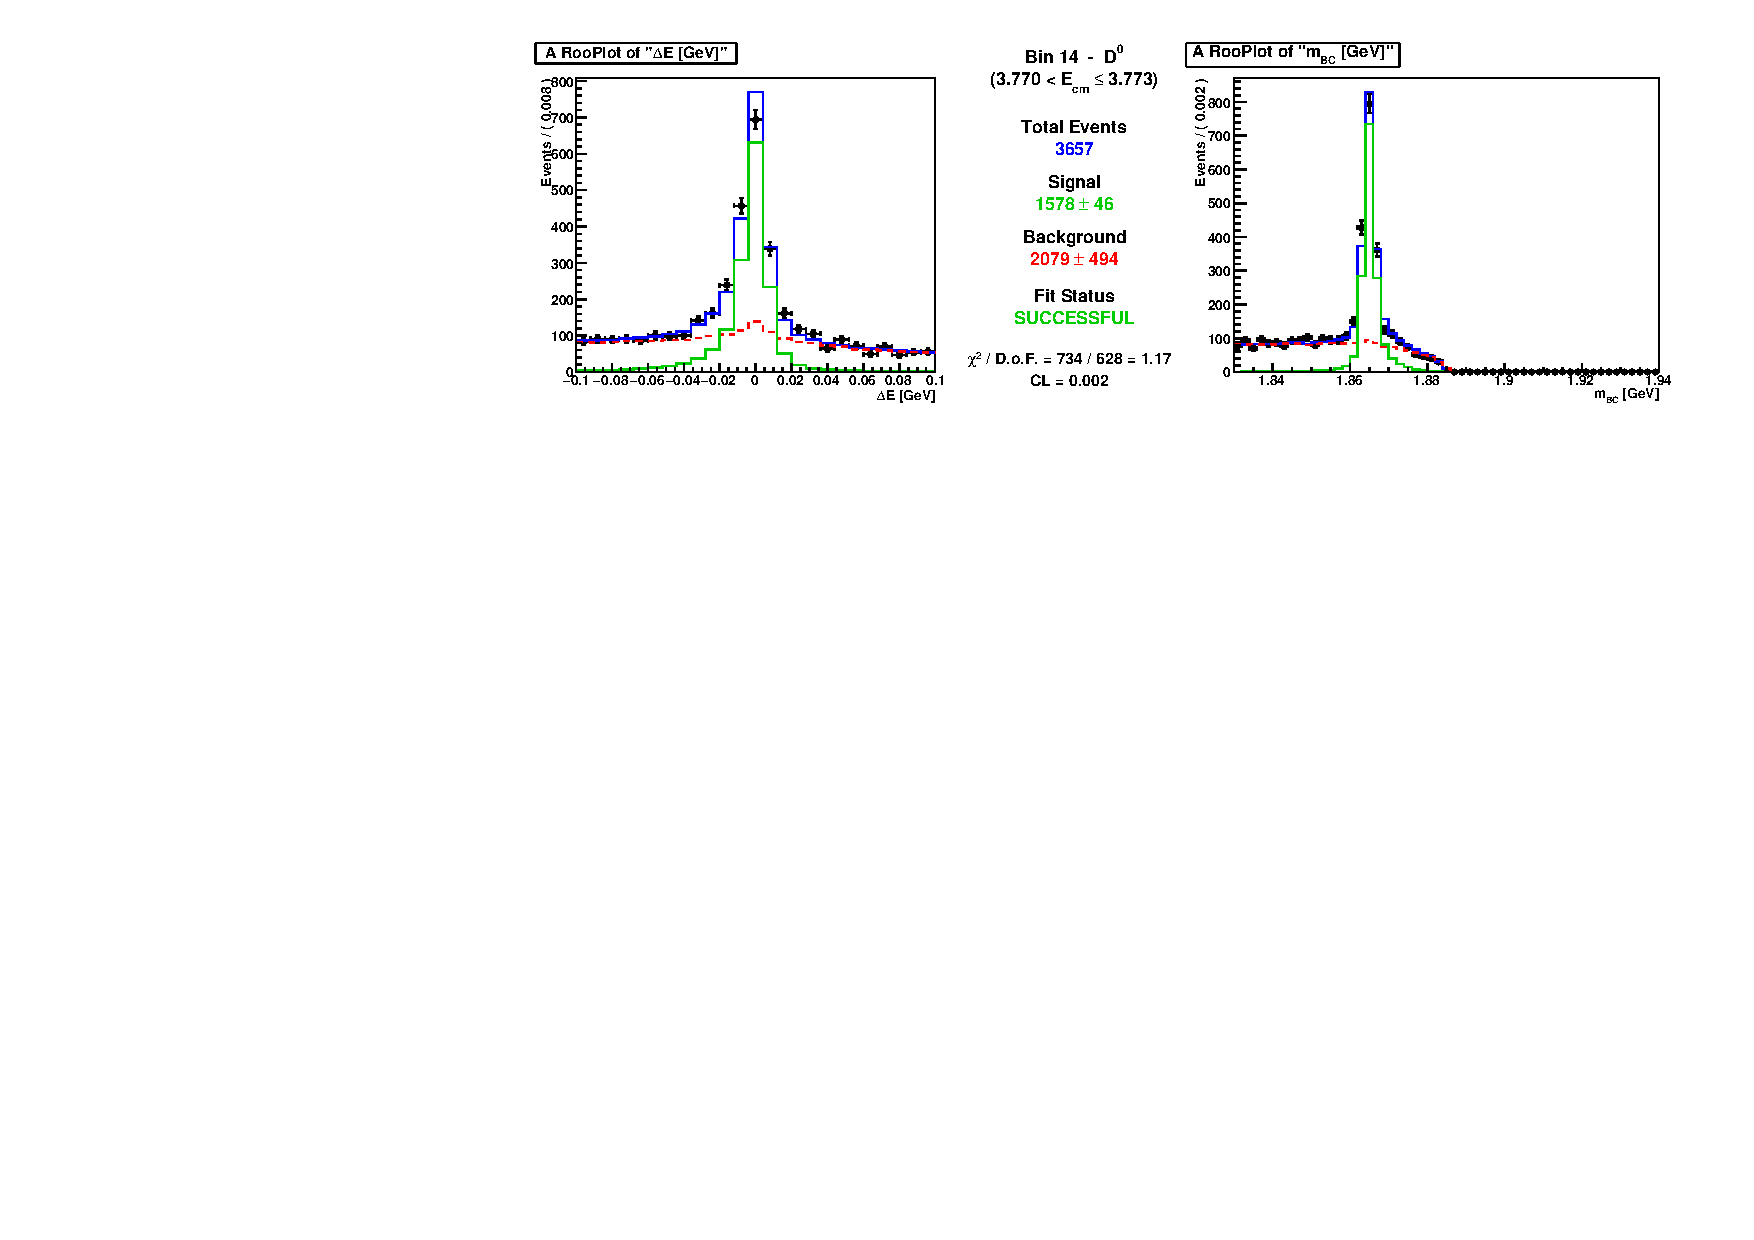
\includegraphics[scale=0.75]{figures/plots/fit_results/D0_bin_14.pdf}
\caption{An example 2D ($\DeltaE$ vs. $\mbc$) signal fit.}{The covers $\DO$ events in the region $\SI{3.774}{\GeV} \leq \Ecm < \SI{3.777}{\GeV}$.
The data points (black) are fitted by the total MC shape (blue), which is the sum of the signal (green) and background (red) components.}
\label{fig:example_fit}
\end{figure}

\pagebreak


\section{Efficiency Correction}
\label{sec:efficiency}

In addition to the parameters gathered by \DTagAlg, truth information was taken from the generic $\DDbar$ samples to determine the mode-by-mode reconstruction efficiencies.
To be deemed proper, a reconstruction must pass not only the standard $\Dtag$ cuts, but also match the generator information for the event.
This process removes backgrounds contributed by modes with similar constituents that tend to peak in the signal region.
The total number of proper $\Dtag$ reconstructions is then divided by the number of $\D$ particles generated for each mode, and the mode-by-mode efficiencies are weighted by the world-average (PDG) branching ratios \cite{ref:Olive:2014} to determine the overall efficiency ($\epsilon_{\D}$) for each of $\DO$ and $\Dp$:
\beq
\label{eq:DDbar_eff}
\epsilon_{D} = \sum_i \epsilon_{i \text{ rec}} \, \mathcal{B}_i = \sum_i \left( \frac{ N_{i \text{ prop}} }{ N_{i \text{ gen}} } \right) \mathcal{B}_i.
\eeq
Each $\DO$ efficiency also includes the corresponding DCSD terms for its decay (see \Cref{sec:d_tagging}).

The efficiencies for $\Dp$ and $\DO$ calculated for the total sample are shown for each mode in \Cref{tab:DTag_eff} and \Cref{fig:D_eff_by_mode}.
However, for the determination of the cross section, this procedure was applied separately for each energy bin.
The numbers of proper and generated particles are shown in \Cref{tab:DTag_eff_D0} for $\DO$ and \Cref{tab:DTag_eff_Dp_p1,tab:DTag_eff_Dp_p2} for $\Dp$ while the total efficiencies for both $\DO$ and $\Dp$ are shown in \Cref{tab:DTag_eff_E_bin}.

\begin{table}[h]
\centering
\begin{tabular}{l r@{$\; \pm \;$}l r@{$\; \pm \;$}l}
\hline
Decay Mode ($i$) & \multicolumn{2}{c}{PDG $\mathcal{B}_i$ [\%]} & \multicolumn{2}{c}{MC Efficiency $\epsilon_i$} \\
\hline
$\DOmodeA$ &  3.89 & 0.05 & 0.7002 & 0.0011 \\
$\DOmodeB$ & 13.93 & 0.50 & 0.3794 & 0.0004 \\
$\DOmodeC$ &  8.11 & 0.21 & 0.3988 & 0.0006 \\
\hline
\multicolumn{5}{c}{$\epsilon_{\DO} = (11.245 \pm 0.020)\%$} \\[1pt]
\hline
$\DpmodeA$ &  9.13 & 0.19 & 0.5471 & 0.0007 \\
$\DpmodeB$ &  5.99 & 0.18 & 0.2739 & 0.0006 \\
$\DpmodeC$ &  1.47 & 0.07 & 0.3883 & 0.0014 \\
$\DpmodeD$ &  6.99 & 0.27 & 0.2079 & 0.0005 \\
$\DpmodeE$ &  3.12 & 0.11 & 0.2237 & 0.0007 \\
$\DpmodeF$ &  0.95 & 0.03 & 0.4317 & 0.0018 \\
\hline
\multicolumn{5}{c}{$\epsilon_{\Dp} = (9.770 \pm 0.063)\%$} \\[1pt]
\hline
\end{tabular}
\caption{Mode-by-mode reconstruction efficiencies for $\DO$ and $\Dp$.}
{The values shown are over the entire data sample, while calculations for the cross sections use the values for each energy point individually (see \Cref{tab:DTag_eff_E_bin}). The errors listed for the PDG branching fractions are shown for reference, and are not included in the efficiency errors (see \Cref{ssec:sys_pdg}).}
\label{tab:DTag_eff}
\end{table}


\begin{figure}[H]
\centering
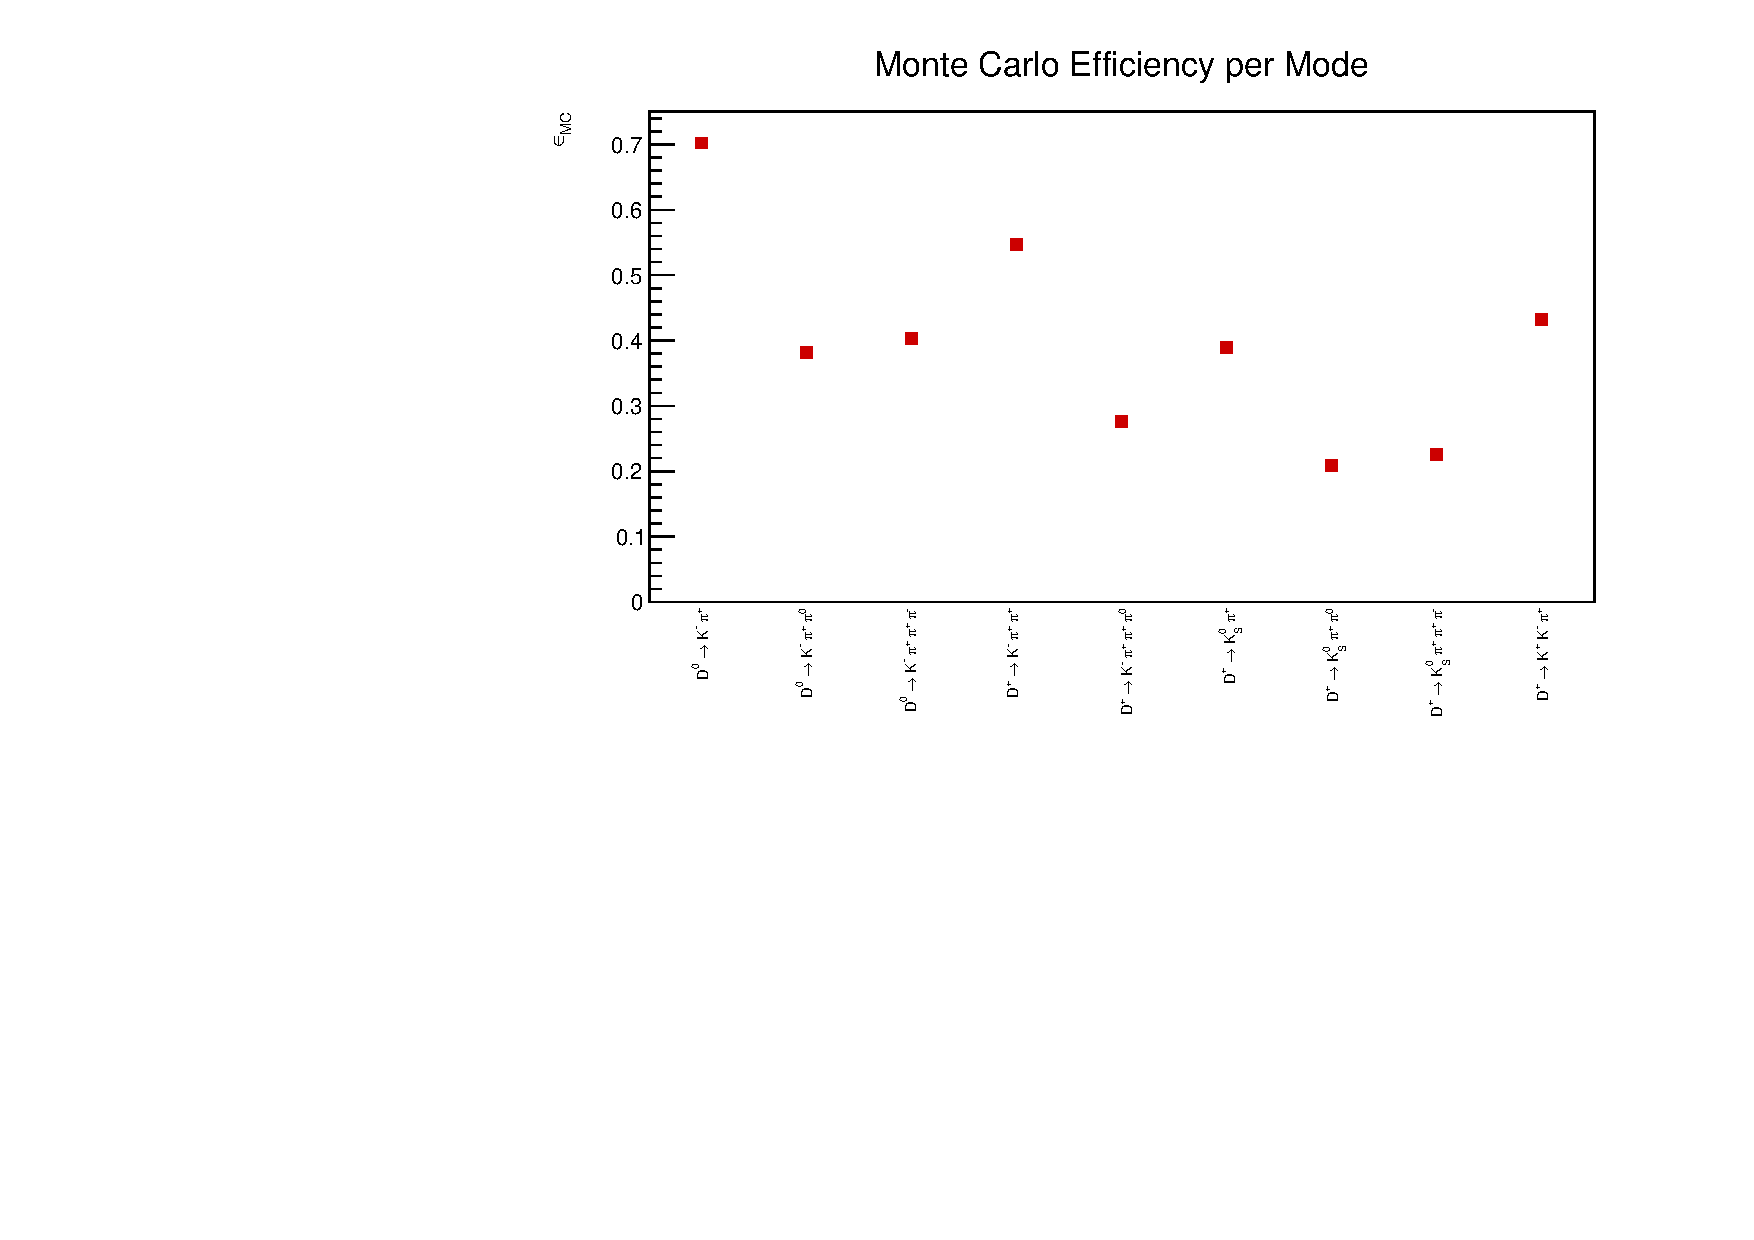
\includegraphics[scale=0.8]{figures/plots/D_eff_by_mode.pdf}
\caption{Mode-by-mode efficiencies for $\DO$ and $\Dp$ determined with signal MC.}
{The error bars are negligible on the scale shown.}
\label{fig:D_eff_by_mode}
\end{figure}



\begin{table}[H]
\renewcommand\arraystretch{1.0}
\centering
\begin{tabular}{c|C{1cm}C{1cm}C{1cm}|C{1cm}C{1cm}C{1cm}|C{1cm}C{1cm}C{1cm}}
\hline
Bin & \multicolumn{3}{c|}{$\DOmodeA$} & \multicolumn{3}{c|}{$\DOmodeB$} & \multicolumn{3}{c}{$\DOmodeC$} \\
& $\Nprop$ & $\Ngen$ & $\epsilon_{\text{rec}}$ & $\Nprop$ & $\Ngen$ & $\epsilon_{\text{rec}}$ & $\Nprop$ & $\Ngen$ & $\epsilon_{\text{rec}}$ \\
\hline
 0 & 11197 & 15757 & 0.711 & 21600 & 55815 & 0.387 & 13592 & 33714 & 0.403 \\
 1 & 11266 & 15713 & 0.717 & 21735 & 56189 & 0.387 & 13651 & 33621 & 0.406 \\
 2 & 11065 & 15557 & 0.711 & 21683 & 55791 & 0.389 & 13984 & 33431 & 0.418 \\
 3 & 10748 & 15501 & 0.693 & 21114 & 55767 & 0.379 & 13168 & 33505 & 0.393 \\
 4 & 11176 & 15779 & 0.708 & 21922 & 55873 & 0.392 & 13613 & 33410 & 0.407 \\
 5 & 10984 & 15722 & 0.699 & 21366 & 56027 & 0.381 & 13483 & 33748 & 0.400 \\
 6 & 10837 & 15507 & 0.699 & 21144 & 55551 & 0.381 & 13738 & 33639 & 0.408 \\
 7 & 10707 & 15645 & 0.684 & 20889 & 56193 & 0.372 & 13074 & 33494 & 0.390 \\
 8 & 11031 & 15585 & 0.708 & 21788 & 55891 & 0.390 & 13967 & 33826 & 0.413 \\
 9 & 10994 & 15485 & 0.710 & 21978 & 56012 & 0.392 & 14020 & 33601 & 0.417 \\
10 & 10952 & 15497 & 0.707 & 21400 & 56126 & 0.381 & 13727 & 33591 & 0.409 \\
11 & 11025 & 15535 & 0.710 & 21700 & 55919 & 0.388 & 13980 & 33706 & 0.415 \\
12 & 10909 & 15593 & 0.700 & 21713 & 55876 & 0.389 & 13787 & 33335 & 0.414 \\
13 & 11088 & 15826 & 0.701 & 21696 & 55758 & 0.389 & 14013 & 33805 & 0.415 \\
14 & 10975 & 15620 & 0.703 & 21576 & 55591 & 0.388 & 14039 & 33581 & 0.418 \\
15 & 10965 & 15672 & 0.700 & 21501 & 55647 & 0.386 & 13777 & 33644 & 0.409 \\
16 & 10803 & 15438 & 0.700 & 21505 & 55667 & 0.386 & 13832 & 33822 & 0.409 \\
17 & 10913 & 15473 & 0.705 & 21574 & 56023 & 0.385 & 14163 & 34131 & 0.415 \\
18 & 11156 & 15856 & 0.704 & 21461 & 55706 & 0.385 & 13725 & 33321 & 0.412 \\
19 & 11124 & 15728 & 0.707 & 21775 & 56192 & 0.388 & 13930 & 33935 & 0.410 \\
20 & 10837 & 15530 & 0.698 & 21149 & 55737 & 0.379 & 13883 & 33703 & 0.412 \\
21 & 10756 & 15397 & 0.699 & 21212 & 55815 & 0.380 & 13577 & 33907 & 0.400 \\
22 & 10986 & 15582 & 0.705 & 21178 & 56343 & 0.376 & 13352 & 33773 & 0.395 \\
23 & 11147 & 15861 & 0.703 & 21088 & 56167 & 0.375 & 13200 & 33680 & 0.392 \\
24 & 10785 & 15633 & 0.690 & 20763 & 55952 & 0.371 & 12651 & 33660 & 0.376 \\
25 & 10972 & 15490 & 0.708 & 20687 & 55957 & 0.370 & 12841 & 33512 & 0.383 \\
26 & 11016 & 15645 & 0.704 & 20707 & 55785 & 0.371 & 12563 & 33615 & 0.374 \\
27 & 10800 & 15420 & 0.700 & 20244 & 55748 & 0.363 & 12362 & 33359 & 0.371 \\
28 & 10939 & 15694 & 0.697 & 20077 & 55550 & 0.361 & 12507 & 33497 & 0.373 \\
29 & 10839 & 15689 & 0.691 & 20685 & 56386 & 0.367 & 12575 & 33551 & 0.375 \\
30 & 10798 & 15766 & 0.685 & 20238 & 55433 & 0.365 & 12526 & 33885 & 0.370 \\
31 & 10568 & 15438 & 0.685 & 20533 & 55825 & 0.368 & 12901 & 33745 & 0.382 \\
32 & 10820 & 15679 & 0.690 & 20706 & 55823 & 0.371 & 13155 & 33810 & 0.389 \\
33 & 10643 & 15736 & 0.676 & 20488 & 55672 & 0.368 & 12875 & 33547 & 0.384 \\
\hline
\end{tabular}
\caption{Numbers of proper and generated particles for $\DO$.}
{The mode-by-mode numbers of particles used in the efficiency calculations for $\DOmodeA, \DOmodeB,$ and $\DOmodeC$.}
\label{tab:DTag_eff_D0}
\end{table}


\begin{table}[H]
\renewcommand\arraystretch{1.0}
\centering
\begin{tabular}{c|C{1cm}C{1cm}C{1cm}|C{1cm}C{1cm}C{1cm}|C{1cm}C{1cm}C{1cm}}
\hline
Bin & \multicolumn{3}{c|}{$\DpmodeA$} & \multicolumn{3}{c|}{$\DpmodeB$} & \multicolumn{3}{c}{$\DpmodeC$} \\
& $\Nprop$ & $\Ngen$ & $\epsilon_{\text{rec}}$ & $\Nprop$ & $\Ngen$ & $\epsilon_{\text{rec}}$ & $\Nprop$ & $\Ngen$ & $\epsilon_{\text{rec}}$ \\
\hline
 2 & 20643 & 37609 & 0.549 & 6853 & 24250 & 0.283 & 2302 & 5900 & 0.390 \\
 3 & 19935 & 37582 & 0.530 & 6569 & 24235 & 0.271 & 2335 & 6114 & 0.382 \\
 4 & 20859 & 37915 & 0.550 & 6653 & 24216 & 0.275 & 2291 & 5879 & 0.390 \\
 5 & 20193 & 37647 & 0.536 & 6611 & 24051 & 0.275 & 2292 & 5965 & 0.384 \\
 6 & 20484 & 37814 & 0.542 & 6616 & 24184 & 0.274 & 2292 & 5924 & 0.387 \\
 7 & 19635 & 37462 & 0.524 & 6411 & 24708 & 0.259 & 2127 & 5815 & 0.366 \\
 8 & 20876 & 37758 & 0.553 & 6867 & 24343 & 0.282 & 2328 & 5841 & 0.399 \\
 9 & 20873 & 37739 & 0.553 & 6754 & 24284 & 0.278 & 2377 & 5911 & 0.402 \\
10 & 20571 & 37487 & 0.549 & 6604 & 24249 & 0.272 & 2360 & 6010 & 0.393 \\
11 & 20669 & 37468 & 0.552 & 6818 & 24268 & 0.281 & 2296 & 5904 & 0.389 \\
12 & 20843 & 37838 & 0.551 & 6783 & 24247 & 0.280 & 2401 & 6074 & 0.395 \\
13 & 20486 & 37286 & 0.549 & 6942 & 24582 & 0.282 & 2335 & 6184 & 0.378 \\
14 & 20935 & 37961 & 0.551 & 6836 & 24467 & 0.279 & 2282 & 5963 & 0.383 \\
15 & 20543 & 37458 & 0.548 & 6769 & 24135 & 0.280 & 2295 & 5889 & 0.390 \\
16 & 20713 & 37543 & 0.552 & 6758 & 24376 & 0.277 & 2356 & 5921 & 0.398 \\
17 & 21016 & 37757 & 0.557 & 6949 & 24470 & 0.284 & 2302 & 5903 & 0.390 \\
18 & 21123 & 38024 & 0.556 & 6635 & 24111 & 0.275 & 2320 & 5889 & 0.394 \\
19 & 20708 & 37357 & 0.554 & 6662 & 24240 & 0.275 & 2204 & 5855 & 0.376 \\
20 & 20760 & 37761 & 0.550 & 6768 & 24395 & 0.277 & 2263 & 5883 & 0.385 \\
21 & 20860 & 37893 & 0.550 & 6668 & 24216 & 0.275 & 2296 & 5996 & 0.383 \\
22 & 20827 & 37820 & 0.551 & 6673 & 24421 & 0.273 & 2353 & 5997 & 0.392 \\
23 & 20796 & 37554 & 0.554 & 6723 & 24377 & 0.276 & 2290 & 5957 & 0.384 \\
24 & 20058 & 37410 & 0.536 & 6415 & 24310 & 0.264 & 2341 & 5966 & 0.392 \\
25 & 20677 & 37552 & 0.551 & 6462 & 24245 & 0.267 & 2364 & 5987 & 0.395 \\
26 & 20300 & 37491 & 0.541 & 6539 & 24405 & 0.268 & 2356 & 5993 & 0.393 \\
27 & 20754 & 37704 & 0.550 & 6530 & 24295 & 0.269 & 2288 & 5969 & 0.383 \\
28 & 20213 & 37428 & 0.540 & 6362 & 24146 & 0.263 & 2341 & 5988 & 0.391 \\
29 & 20565 & 37545 & 0.548 & 6495 & 24257 & 0.268 & 2262 & 5916 & 0.382 \\
30 & 20313 & 37773 & 0.538 & 6535 & 24167 & 0.270 & 2323 & 6075 & 0.382 \\
31 & 20322 & 37280 & 0.545 & 6566 & 24389 & 0.269 & 2378 & 5927 & 0.401 \\
32 & 20883 & 37992 & 0.550 & 6594 & 24249 & 0.272 & 2306 & 5855 & 0.394 \\
33 & 20645 & 37738 & 0.547 & 6560 & 24195 & 0.271 & 2269 & 5945 & 0.382 \\
\hline
\end{tabular}
\caption{Numbers of proper and generated particles for $\Dp$ (part 1).}
{The mode-by-mode numbers of particles used in the efficiency calculations for $\DpmodeA, \DpmodeB,$ and $\DpmodeC$.}
\label{tab:DTag_eff_Dp_p1}
\end{table}


\begin{table}[H]
\renewcommand\arraystretch{1.0}
\centering
\begin{tabular}{c|C{1cm}C{1cm}C{1cm}|C{1cm}C{1cm}C{1cm}|C{1cm}C{1cm}C{1cm}}
\hline
Bin & \multicolumn{3}{c|}{$\DpmodeD$} & \multicolumn{3}{c|}{$\DpmodeE$} & \multicolumn{3}{c}{$\DpmodeF$} \\
& $\Nprop$ & $\Ngen$ & $\epsilon_{\text{rec}}$ & $\Nprop$ & $\Ngen$ & $\epsilon_{\text{rec}}$ & $\Nprop$ & $\Ngen$ & $\epsilon_{\text{rec}}$ \\
\hline

 2 & 5742 & 27235 & 0.211 & 3562 & 15019 & 0.237 & 1720 & 4019 & 0.428 \\
 3 & 5668 & 27699 & 0.205 & 3169 & 14877 & 0.213 & 1637 & 3970 & 0.412 \\
 4 & 5710 & 27527 & 0.207 & 3358 & 14750 & 0.228 & 1791 & 4016 & 0.446 \\
 5 & 5614 & 27654 & 0.203 & 3282 & 14696 & 0.223 & 1748 & 3981 & 0.439 \\
 6 & 5656 & 27475 & 0.206 & 3392 & 14823 & 0.229 & 1771 & 4075 & 0.435 \\
 7 & 5481 & 27597 & 0.199 & 3293 & 14860 & 0.222 & 1593 & 3951 & 0.403 \\
 8 & 5827 & 27975 & 0.208 & 3462 & 15035 & 0.230 & 1736 & 4042 & 0.429 \\
 9 & 6003 & 27589 & 0.218 & 3427 & 14906 & 0.230 & 1716 & 3940 & 0.436 \\
10 & 5722 & 27751 & 0.206 & 3327 & 14854 & 0.224 & 1690 & 3941 & 0.429 \\
11 & 5888 & 27649 & 0.213 & 3385 & 14837 & 0.228 & 1672 & 3930 & 0.425 \\
12 & 5731 & 27651 & 0.207 & 3370 & 14926 & 0.226 & 1718 & 3889 & 0.442 \\
13 & 5792 & 27618 & 0.210 & 3336 & 14669 & 0.227 & 1696 & 3958 & 0.428 \\
14 & 5745 & 27608 & 0.208 & 3288 & 14702 & 0.224 & 1712 & 3904 & 0.439 \\
15 & 5832 & 27480 & 0.212 & 3384 & 14808 & 0.229 & 1649 & 3855 & 0.428 \\
16 & 5891 & 27758 & 0.212 & 3443 & 14845 & 0.232 & 1783 & 3947 & 0.452 \\
17 & 5954 & 27639 & 0.215 & 3484 & 14910 & 0.234 & 1804 & 3941 & 0.458 \\
18 & 5875 & 27669 & 0.212 & 3366 & 14913 & 0.226 & 1700 & 3968 & 0.428 \\
19 & 5773 & 27838 & 0.207 & 3371 & 14782 & 0.228 & 1766 & 4037 & 0.437 \\
20 & 6024 & 28019 & 0.215 & 3367 & 14801 & 0.227 & 1709 & 3903 & 0.438 \\
21 & 5804 & 27645 & 0.210 & 3306 & 14819 & 0.223 & 1688 & 3863 & 0.437 \\
22 & 5893 & 27692 & 0.213 & 3304 & 14949 & 0.221 & 1741 & 3975 & 0.438 \\
23 & 5780 & 27865 & 0.207 & 3313 & 14981 & 0.221 & 1670 & 3891 & 0.429 \\
24 & 5623 & 27811 & 0.202 & 3161 & 14867 & 0.213 & 1667 & 3954 & 0.422 \\
25 & 5684 & 27490 & 0.207 & 3250 & 14794 & 0.220 & 1711 & 3966 & 0.431 \\
26 & 5704 & 27829 & 0.205 & 3137 & 14811 & 0.212 & 1641 & 3958 & 0.415 \\
27 & 5630 & 27497 & 0.205 & 3132 & 14881 & 0.210 & 1678 & 3972 & 0.422 \\
28 & 5724 & 28006 & 0.204 & 3271 & 14828 & 0.221 & 1690 & 3931 & 0.430 \\
29 & 5693 & 27554 & 0.207 & 3272 & 15009 & 0.218 & 1772 & 3994 & 0.444 \\
30 & 5574 & 27717 & 0.201 & 3308 & 14730 & 0.225 & 1673 & 4026 & 0.416 \\
31 & 5556 & 27556 & 0.202 & 3288 & 15049 & 0.218 & 1746 & 3965 & 0.440 \\
32 & 5785 & 27634 & 0.209 & 3259 & 14840 & 0.220 & 1680 & 3923 & 0.428 \\
33 & 5653 & 27528 & 0.205 & 3287 & 14959 & 0.220 & 1734 & 4031 & 0.430 \\
\hline
\end{tabular}
\caption{Numbers of proper and generated particles for $\Dp$ (part 2).}
{The mode-by-mode numbers of particles used in the efficiency calculations for $\DpmodeD, \DpmodeE,$ and $\DpmodeF$.}
\label{tab:DTag_eff_Dp_p2}
\end{table}


\begin{table}[H]
\centering
\renewcommand\arraystretch{1.0}
\begin{tabular}{c r@{$\; \pm \;$}l r@{$\; \pm \;$}l}
\hline
$E_{\text{bin}}$ & \multicolumn{2}{c}{$\epsilon_{\DO}$} & \multicolumn{2}{c}{$\epsilon_{\Dp}$} \\
\hline
 0 & 0.1146 & 0.0005 & \multicolumn{2}{c}{-} \\
 1 & 0.1151 & 0.0005 & \multicolumn{2}{c}{-} \\
 2 & 0.1161 & 0.0005 & 0.0990 & 0.0005 \\
 3 & 0.1119 & 0.0005 & 0.0952 & 0.0005 \\
 4 & 0.1156 & 0.0005 & 0.0983 & 0.0005 \\
 5 & 0.1131 & 0.0005 & 0.0964 & 0.0005 \\
 6 & 0.1137 & 0.0005 & 0.0972 & 0.0005 \\
 7 & 0.1104 & 0.0005 & 0.0934 & 0.0005 \\
 8 & 0.1157 & 0.0005 & 0.0991 & 0.0005 \\
 9 & 0.1165 & 0.0005 & 0.0996 & 0.0005 \\
10 & 0.1141 & 0.0005 & 0.0977 & 0.0005 \\
11 & 0.1157 & 0.0005 & 0.0990 & 0.0005 \\
12 & 0.1152 & 0.0005 & 0.0986 & 0.0005 \\
13 & 0.1154 & 0.0005 & 0.0985 & 0.0005 \\
14 & 0.1157 & 0.0005 & 0.0984 & 0.0005 \\
15 & 0.1146 & 0.0005 & 0.0986 & 0.0005 \\
16 & 0.1146 & 0.0005 & 0.0992 & 0.0005 \\
17 & 0.1151 & 0.0005 & 0.1003 & 0.0005 \\
18 & 0.1148 & 0.0005 & 0.0990 & 0.0005 \\
19 & 0.1151 & 0.0005 & 0.0984 & 0.0005 \\
20 & 0.1138 & 0.0005 & 0.0988 & 0.0005 \\
21 & 0.1129 & 0.0005 & 0.0982 & 0.0005 \\
22 & 0.1122 & 0.0005 & 0.0984 & 0.0005 \\
23 & 0.1118 & 0.0005 & 0.0982 & 0.0005 \\
24 & 0.1094 & 0.0005 & 0.0953 & 0.0005 \\
25 & 0.1105 & 0.0005 & 0.0975 & 0.0005 \\
26 & 0.1098 & 0.0005 & 0.0962 & 0.0005 \\
27 & 0.1082 & 0.0005 & 0.0969 & 0.0005 \\
28 & 0.1081 & 0.0005 & 0.0961 & 0.0005 \\
29 & 0.1087 & 0.0005 & 0.0971 & 0.0005 \\
30 & 0.1078 & 0.0005 & 0.0959 & 0.0005 \\
31 & 0.1092 & 0.0005 & 0.0969 & 0.0005 \\
32 & 0.1104 & 0.0005 & 0.0978 & 0.0005 \\
33 & 0.1090 & 0.0005 & 0.0971 & 0.0005 \\
\hline
\end{tabular}
\caption{The overall reconstruction efficiency of $\DO$ and $\Dp$ for each energy bin.}
{These values are used to calculate the corresponding cross sections at each energy point.  The listed errors are statistical only.}
\label{tab:DTag_eff_E_bin}
\end{table}


\subsection{$\sCP$ Violation Correction}
\label{ssec:cp_correction}

Due to $\sCP$ violation in the $\DO \aDO$ system, each of the neutral decay modes must be corrected to account for quantum correlations arising from production through a $J^{PC} = 1^{--}$ state.
This is done by applying scaling factors to the efficiency for each of the three modes used in reconstruction.
The corrections are parameterized for each mode ($m$) by the following form \cite{ref:Asner:2008}:
\beq
\label{eq:qc}
\alpha_{\DO \rightarrow m} = 1 + r_m^2 + 2 \times y \times r_m \times R_m \times \cos(\delta_m).
\eeq
Here, $r_m$ and $\delta_m$ represent the relative magnitudes and phases between the Cabbibo-favored and doubly-Cabbibo-suppressed modes, respectively, while the factor of $R_m$ represents a coherence factor characterizing the variation of $\delta_m$ over phase space.
Note, there is no such variation for a two-body decay (like $\DOmodeA$), so $R_{\DOmodeA} = 1$.
The value of $y$ represents the difference in total width components of the $\DO \aDO$ system, $y = (\Gamma_2 - \Gamma_1) / (\Gamma_2 + \Gamma_1)$, where 1 and 2 represent the $\sCP$-odd and $\sCP$-even states, respectively.

The mode-dependent values for these factors are listed in \Cref{tab:qc_factors}.
These are taken from the $CPV$-allowed values in \cite{ref:HFAG:2015} for $\DOmodeA$, and from \cite{ref:Evans:2016} for $\DOmodeB$ and $\DOmodeC$.
The value $y = 0.0066^{+0.0007}_{-0.0010}$ is also from \cite{ref:HFAG:2015}, and is the same for all modes.
After applying each of the mode-dependent corrections, the efficiency for the full sample changes from $\epsilon_{\DO} = (11.320 \pm 0.213)\%$ to $\epsilon_{\DO} = (11.352 \pm 0.213)\%$, and similarly for the efficiencies of each $\Ecm$ bin.

\begin{table}[H]
\renewcommand\arraystretch{1.0}
\begin{tabular}{l|r@{$\;\pm\;$}l r@{~}l r@{~}l|r@{~}l}
\hline 
\multicolumn{1}{c|}{Mode}  & \multicolumn{2}{c}{$r_m$} & \multicolumn{2}{c}{$R_m$} & \multicolumn{2}{c|}{$\delta_m$ [\si{^\circ}]} & \multicolumn{2}{c}{$\alpha_m$} \\
\hline
$\DOmodeA$ & 0.0591 & 0.0063 & \multicolumn{2}{c}{1}         &  11.8 & $^{+\;\pp 9.5}_{-\;14.7}$ & 1.00426 & $ \pm\; 0.00083$             \\
$\DOmodeB$ & 0.0447 & 0.0012 & 0.81 & $\pm\; 0.06$           &  18   & $^{+\;   14  }_{-\;15  }$ & 1.00248 & $ \pm\; 0.00014$             \\
$\DOmodeC$ & 0.0549 & 0.0006 & 0.43 & $^{+\;0.17}_{-\;0.13}$ & -52   & $^{+\;   28  }_{-\;17  }$ & 1.00270 & $^{+\;0.00014}_{-\;0.00012}$ \\
\hline 
\end{tabular}
\caption{The quantum correlated factors for the $\DO$ modes.}
\label{tab:qc_factors}
\end{table}

\pagebreak


\section{Fitting Procedure}
\label{sec:fitting}

After applying the correction in \Cref{ssec:cp_correction}, the efficiency values (\Cref{tab:DTag_eff_E_bin}) were combined with the luminosity (\Cref{tab:luminosity}) and the signal values from each 2D fit (\Cref{tab:xsec_rc_data}) to determine the cross section at each energy point.  Since each $\psipp$ produces a $\DDbar$ pair, a factor of 2 is included in the denominator to correct for double counting:
\beq
\label{eq:xsec_rc_data}
\sigma_{\DDbar}^{RC}(E_i) = \frac{ N_D(E_i) }{ 2 \, \epsilon_D(E_i) \, \mathcal{L}(E_i) }.
\eeq
The resulting cross sections for $\DO$ and $\Dp$ are shown in \Cref{fig:xsec_rc_data} and \Cref{tab:xsec_rc_data}.


\begin{table}
\centering
\begin{tabular}{c r@{$\;\pm\;$}r r@{$\;\pm\;$}l r@{$\;\pm\;$}r r@{$\;\pm\;$}l}
\hline
$E_{\text{mid}}$ & \multicolumn{2}{c}{$N_{\DO \aDO}$} & \multicolumn{2}{c}{$\sigma^{RC}_{\DO \aDO}$ [\si{\nb}]} & \multicolumn{2}{c}{$N_{\Dp \Dm}$}  & \multicolumn{2}{c}{$\sigma^{RC}_{\Dp \Dm}$ [\si{\nb}]} \\
\hline
3.7342 &   32 &  9 & 0.169 & 0.046 & \multicolumn{2}{c}{-} & \multicolumn{2}{c}{-} \\
3.7368 &   16 &  5 & 0.218 & 0.068 & \multicolumn{2}{c}{-} & \multicolumn{2}{c}{-} \\
3.7447 &  169 & 16 & 0.765 & 0.070 &   28 &  7 & 0.150 & 0.038 \\
3.7483 &  264 & 20 & 0.838 & 0.064 &   96 & 13 & 0.360 & 0.048 \\
3.7501 &  509 & 28 & 0.968 & 0.053 &  196 & 18 & 0.439 & 0.040 \\
3.7517 &  831 & 34 & 1.237 & 0.052 &  329 & 23 & 0.574 & 0.040 \\
3.7534 & 1036 & 38 & 1.377 & 0.051 &  481 & 27 & 0.748 & 0.042 \\
3.7556 & 1182 & 41 & 1.566 & 0.055 &  508 & 28 & 0.797 & 0.045 \\
3.7562 & 1459 & 45 & 1.629 & 0.051 &  701 & 32 & 0.914 & 0.042 \\
3.7592 & 2014 & 52 & 1.948 & 0.052 & 1054 & 39 & 1.192 & 0.045 \\
3.7624 & 2444 & 58 & 2.385 & 0.058 & 1346 & 44 & 1.534 & 0.051 \\
3.7650 & 2062 & 53 & 2.715 & 0.071 & 1223 & 42 & 1.882 & 0.066 \\
3.7676 & 1746 & 48 & 3.102 & 0.087 & 1059 & 39 & 2.200 & 0.081 \\
3.7713 & 1585 & 46 & 3.406 & 0.101 & 1045 & 38 & 2.634 & 0.098 \\
3.7742 & 1569 & 46 & 3.714 & 0.111 & 1103 & 40 & 3.067 & 0.111 \\
3.7775 & 1543 & 46 & 3.692 & 0.111 & 1108 & 39 & 3.078 & 0.111 \\
3.7802 & 1539 & 46 & 3.444 & 0.104 & 1006 & 38 & 2.599 & 0.100 \\
3.7829 & 1381 & 44 & 2.791 & 0.090 &  951 & 38 & 2.206 & 0.088 \\
3.7869 & 1167 & 42 & 1.995 & 0.072 &  821 & 36 & 1.627 & 0.073 \\
3.7891 &  888 & 38 & 1.361 & 0.058 &  656 & 34 & 1.178 & 0.062 \\
3.7926 &  739 & 36 & 0.920 & 0.045 &  475 & 32 & 0.680 & 0.045 \\
3.7970 &  514 & 34 & 0.562 & 0.037 &  329 & 31 & 0.414 & 0.039 \\
3.8003 &  374 & 31 & 0.424 & 0.035 &  186 & 28 & 0.241 & 0.037 \\
3.8024 &  196 & 23 & 0.325 & 0.038 &  125 & 23 & 0.236 & 0.043 \\
3.8070 &  136 & 19 & 0.352 & 0.050 &   97 & 17 & 0.289 & 0.051 \\
3.8093 &   65 & 14 & 0.233 & 0.050 &   32 & 13 & 0.132 & 0.055 \\
3.8135 &   12 & 10 & 0.060 & 0.049 &   26 & 11 & 0.153 & 0.066 \\
3.8153 &    8 &  7 & 0.056 & 0.051 &   12 &  8 & 0.089 & 0.063 \\
3.8229 &   12 &  7 & 0.140 & 0.083 &   15 &  8 & 0.197 & 0.107 \\
3.8320 &    4 &  5 & 0.069 & 0.086 &    3 &  5 & 0.046 & 0.099 \\
3.8390 &   14 &  6 & 0.237 & 0.105 &   14 &  7 & 0.254 & 0.124 \\
3.8494 &   11 &  6 & 0.186 & 0.104 &   10 &  6 & 0.186 & 0.118 \\
3.8555 &   24 &  8 & 0.337 & 0.111 &   17 &  6 & 0.273 & 0.104 \\
3.8632 &   22 &  8 & 0.340 & 0.127 &    6 &  5 & 0.099 & 0.091 \\
\hline
\end{tabular} 
\caption{The $\DDbar$ cross section at each $\Ecm$ point.}
{The numbers of data events observed in each $\Ecm$ bin are also shown.
The uncertainties on the cross sections are statistical only and come from the signal fitting ($N_D$), PDG values (\Cref{tab:DTag_eff}), and MC reconstruction efficiencies (\Cref{tab:DTag_eff_E_bin}).
The values for $N_{\DO \aDO}$ and $N_{\Dp \Dm}$ are taken from the signal fits shown in \Cref{app:D0_signal_fits,app:Dp_signal_fits}.}
\label{tab:xsec_rc_data}
\end{table}


\begin{figure}[h]
\centering
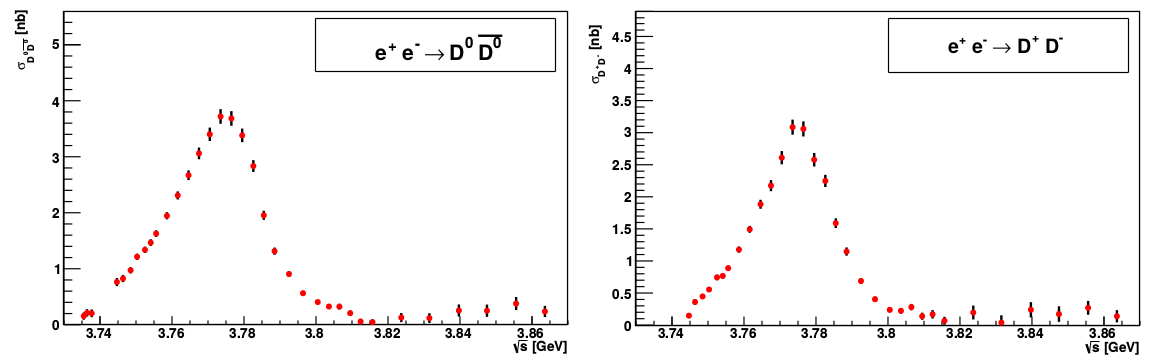
\includegraphics[scale=0.35]{figures/plots/xsec_data.png}
\caption{The measured $\ee \rightarrow \DDbar$ cross sections.}
{The $\DO \aDO$ cross section is shown on the left and $\Dp \Dm$ is shown on the right. }
\label{fig:xsec_rc_data}
\end{figure}


These cross sections are fit to \Cref{eq:xsec_rc_simp} using each form factor choice described in \Cref{sec:form_factors}.
There are four common fit parameters, $\Mpsipp$, $\Gpsipp$, $\Geepsipp$, and $\Ppsipp$, representing the mass, total width, electron partial width, and relative phase to the non-resonant contribution for the $\psipp$, respectively.
The total width corresponds to $\Gamma(M)$ in \Cref{sec:xsec_derivation}.
Two additional parameters are form factor dependent: $F_{NR}$ and $a_{NR}$ for the exponential, or $\Gpsip$ and $F_0$ for the VDM.
For the former, these represent the amplitude and exponent normalization for the non-resonant contribution.
For the latter, these represent the modified total width for the $\psip$ above resonance (see \Cref{sec:form_factors}) and the constant contribution of resonances above the $\psipp$.
The fitting is done simultaneously for $\DO$ and $\Dp$ with identical parameters using TMinuit \cite{ref:TMinuit}.
The minimized $\chi^2$ is the total contribution from both $\DO$ and $\Dp$.  
Results for the Exponential and VDM form factors are shown in \Cref{fig:exp_results,fig:vdm_results}, respectively.


\begin{figure}[H]
\centering
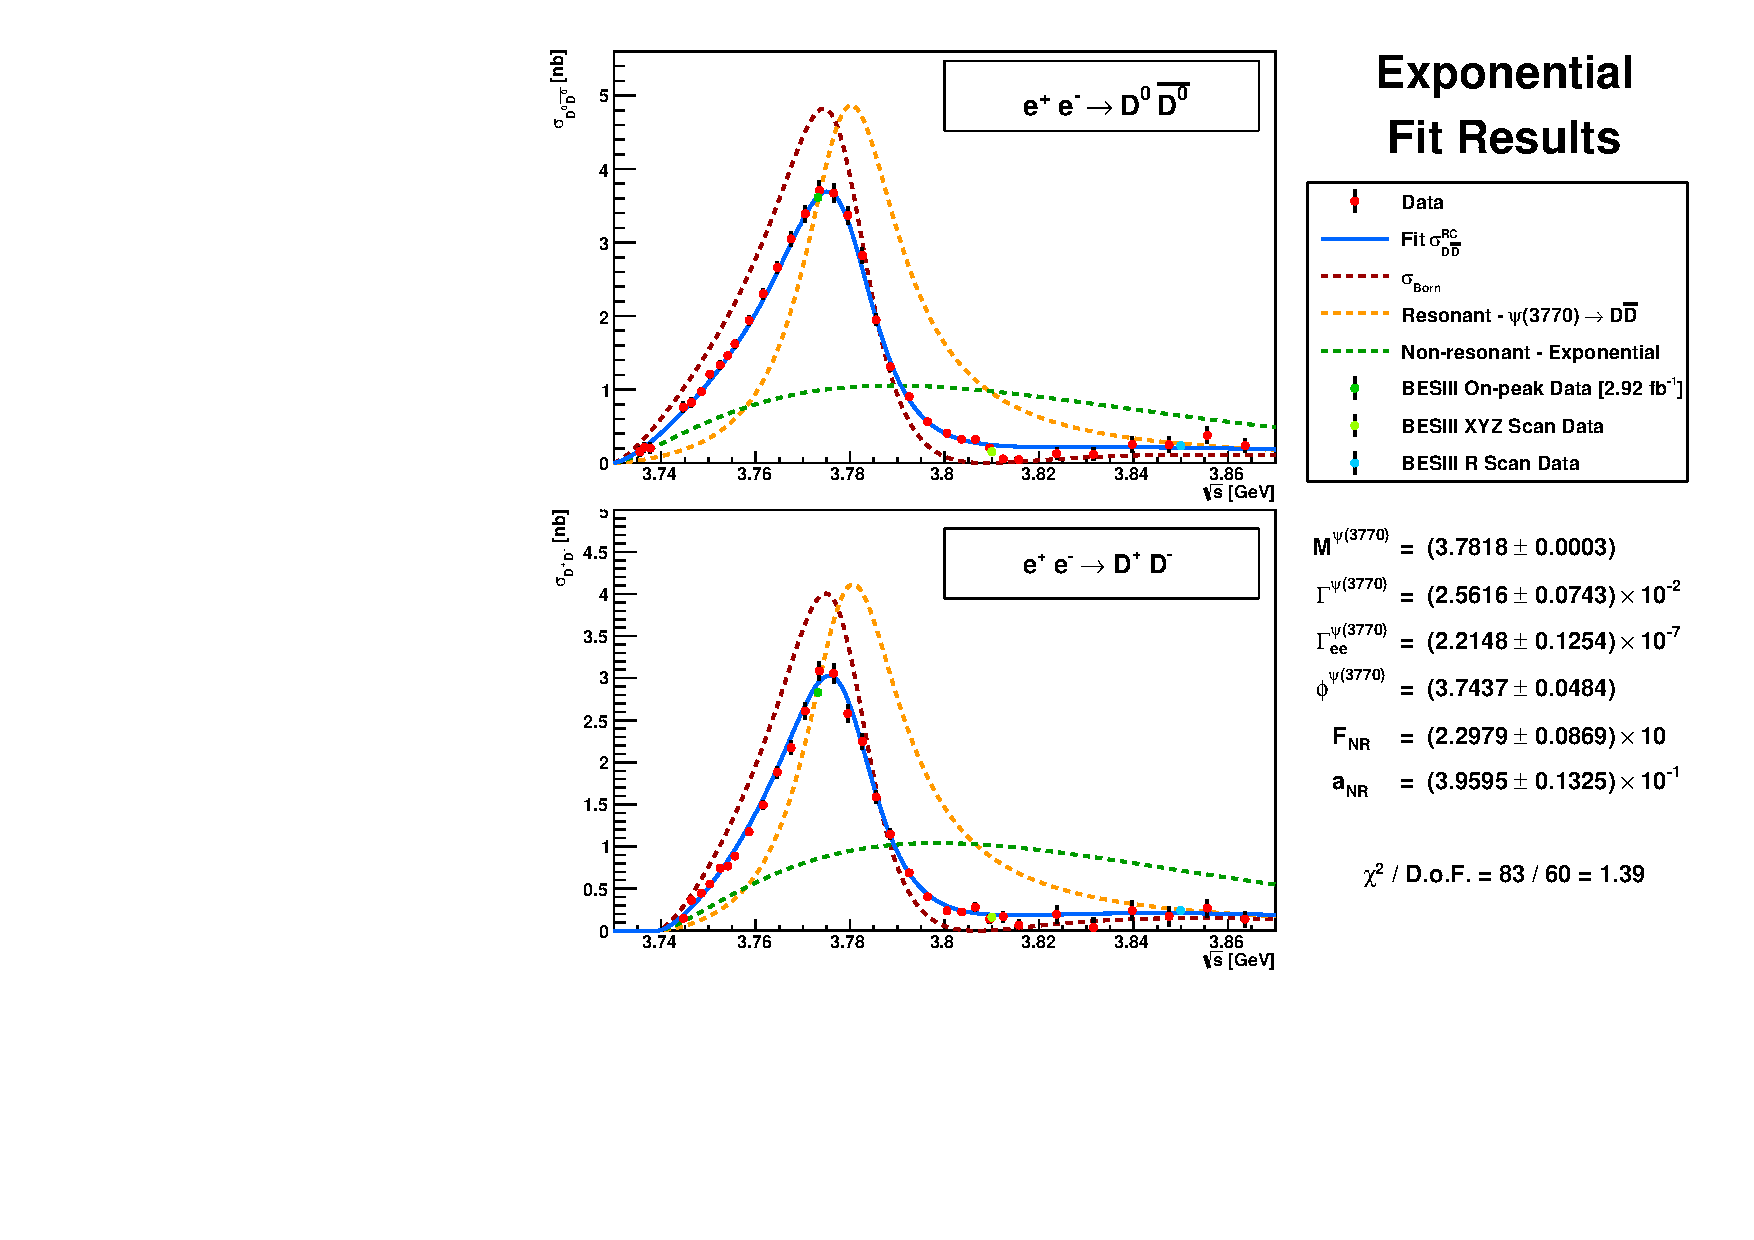
\includegraphics[scale=0.75]{figures/plots/lineshape_exp.pdf}
\caption{The Exponential Model fit results.}
{Both the $\DO$ (top) and the $\Dp$ (bottom) use a fit shape (blue) calculated from \Cref{eq:xsec_rc} using the non-resonant component from \Cref{eq:exp_model}.}
\label{fig:exp_results}
\end{figure}

\begin{figure}[H]
\centering
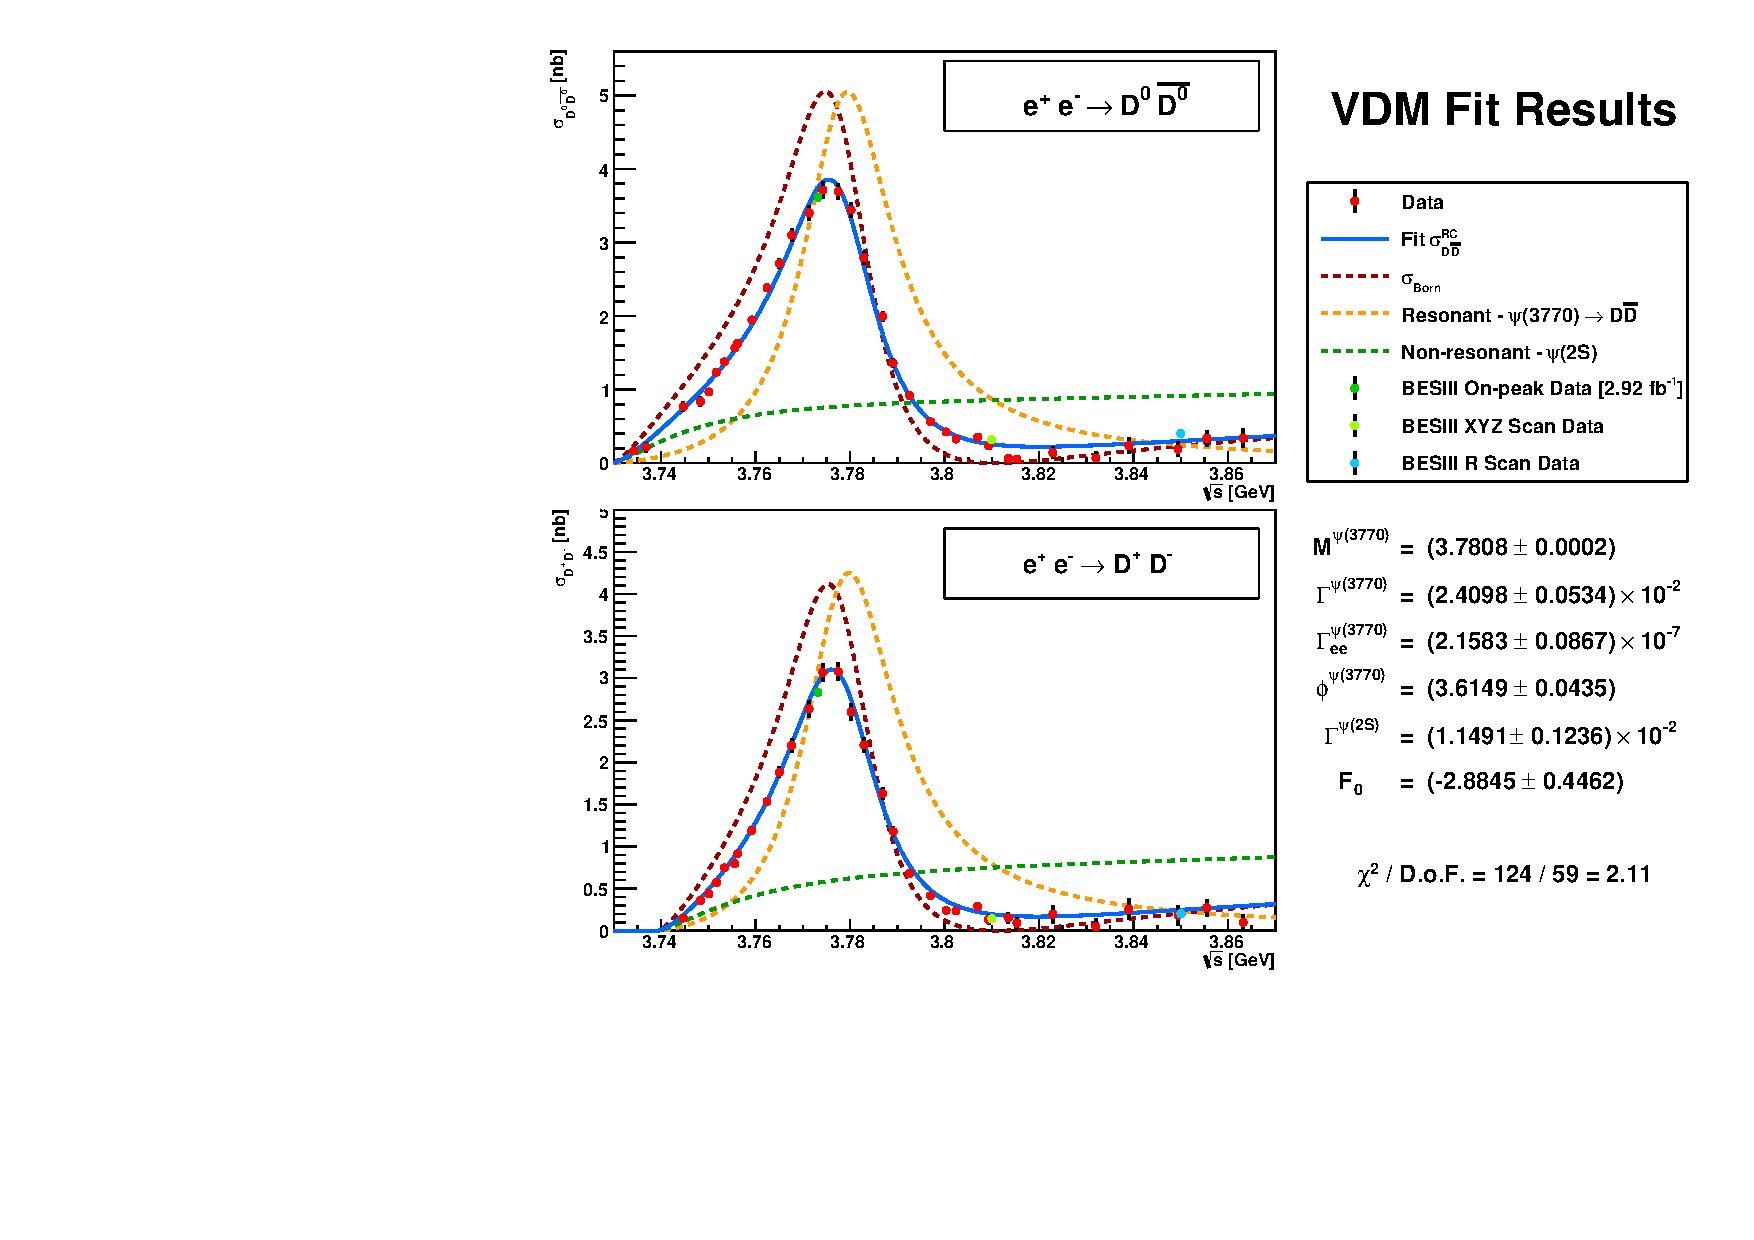
\includegraphics[scale=0.75]{figures/plots/lineshape_vdm.pdf}
\caption{The Vector Dominance Model fit results.}
{Both the $\DO$ (top) and the $\Dp$ (bottom) use a fit shape (blue) calculated from \Cref{eq:xsec_rc} using the non-resonant component from \Cref{eq:vdm_model}.}
\label{fig:vdm_results}
\end{figure}

Both form factor choices show generally good agreement with their theoretical formulation.
While a value of $\chi^2 / \text{ D.o.F. (degrees of freedom)} \approx 2$ is a bit higher than desired, much of this excess is due to a small set of points.
Namely, the two points within \SIrange{3.81}{3.82}{\GeV} for the $\DO$ cross section are well below the predicted shape.
This could indicate the model used in our analysis does not well cover this region, and more information is needed to better understand the shape.
Still, the parameters for the $\psipp$ are heavily dominated by the energy points in the peak region, and the overall consistency shown in this range provides confidence in the values obtained.


\subsection{Coulomb Correction}
\label{ssec:coulomb}

In the development of this analysis, it was discovered that the unmodified theoretical formulation in \Cref{sec:xsec_derivation} did not lead to a successful fit of the $\DDbar$ cross sections, as shown in \Cref{fig:vdm_Coulomb}.
Namely, including the Coulomb effect pulls the $\DO \aDO$ and $\Dp \Dm$ cross sections in opposite directions.
We found the best fits were achieved by altering \Cref{eq:z_Dp} to set the Coulomb factor to 1.
While this disagrees with conventional theoretical wisdom, it is consistent with studies of $\Upsilon(4S) \rightarrow B\overline{B}$ where applying a Coulomb correction for the charged final state also leads to inconsistency with data.

\begin{figure}[H]
\centering
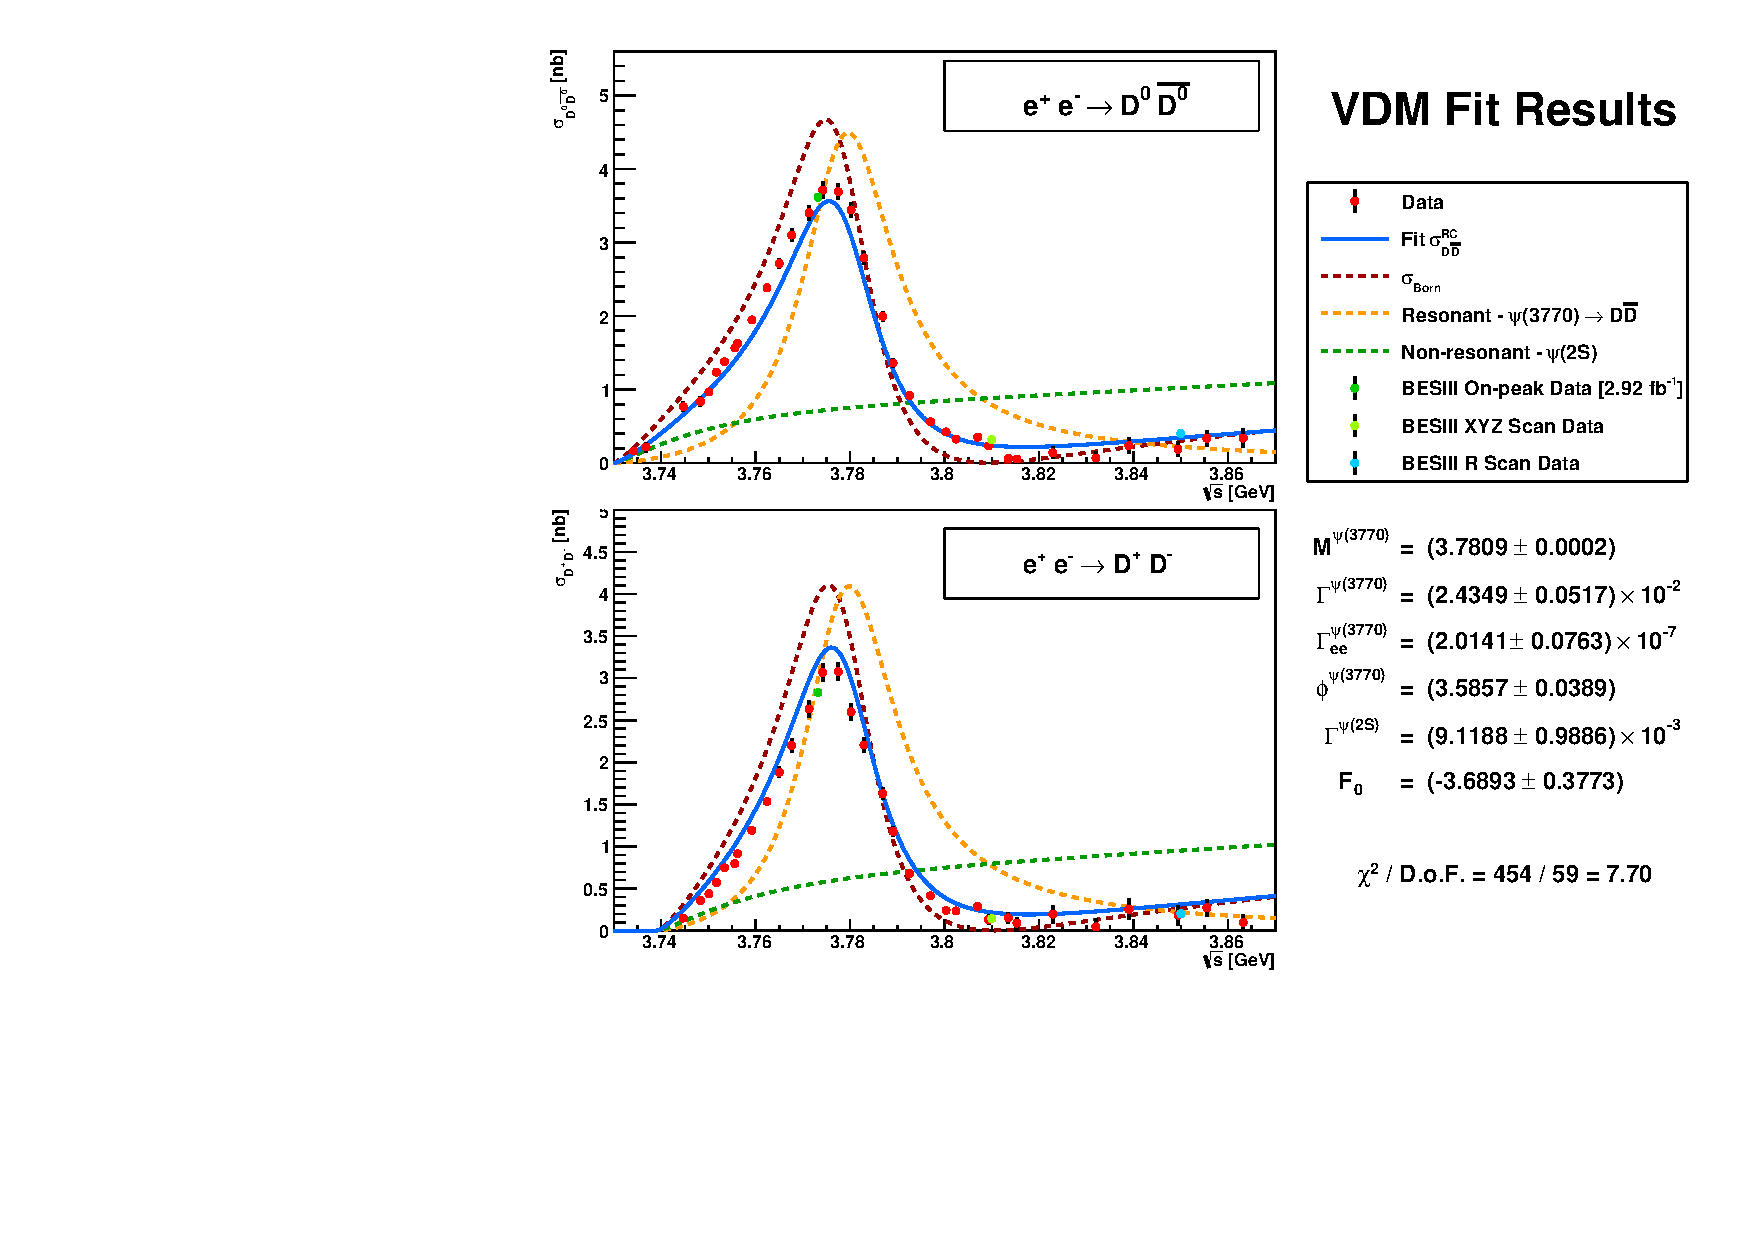
\includegraphics[scale=0.75]{figures/plots/lineshape_vdm_Coulomb.pdf}
\caption{The Vector Dominance Model fit results with Coulomb interactions.}
{Including this factor provides notably worse results than when excluding it (see \Cref{fig:vdm_results}).}
\label{fig:vdm_Coulomb}
\end{figure}

This is most clearly seen in the ratio of $\Dp \Dm$ and $\DO \aDO$ cross sections, shown in \Cref{fig:Coulomb_ratio}, where the `No Coulomb' method sets $\zDD$ in \Cref{eq:xsec_rc_simp,eq:Gamma} to unity, the `Partial Coulomb' sets this factor to unity only for \Cref{eq:xsec_rc_simp}, and the `Full Coulomb' is the default assumption.
Agreement of the measured cross section ratio with the `No Coulomb' calculation is substantially better.
This is also true for the high statistics points measured at the $\psipp$ peak by Derrick Toth \cite{ref:Toth:2014} (light blue).
As the data tend to follow the `No Coulomb' method, we choose this as our nominal method for the results, presented in \Cref{sec:results}.
However, the explanation for this behavior is still undetermined.

\begin{figure}[H]
\centering
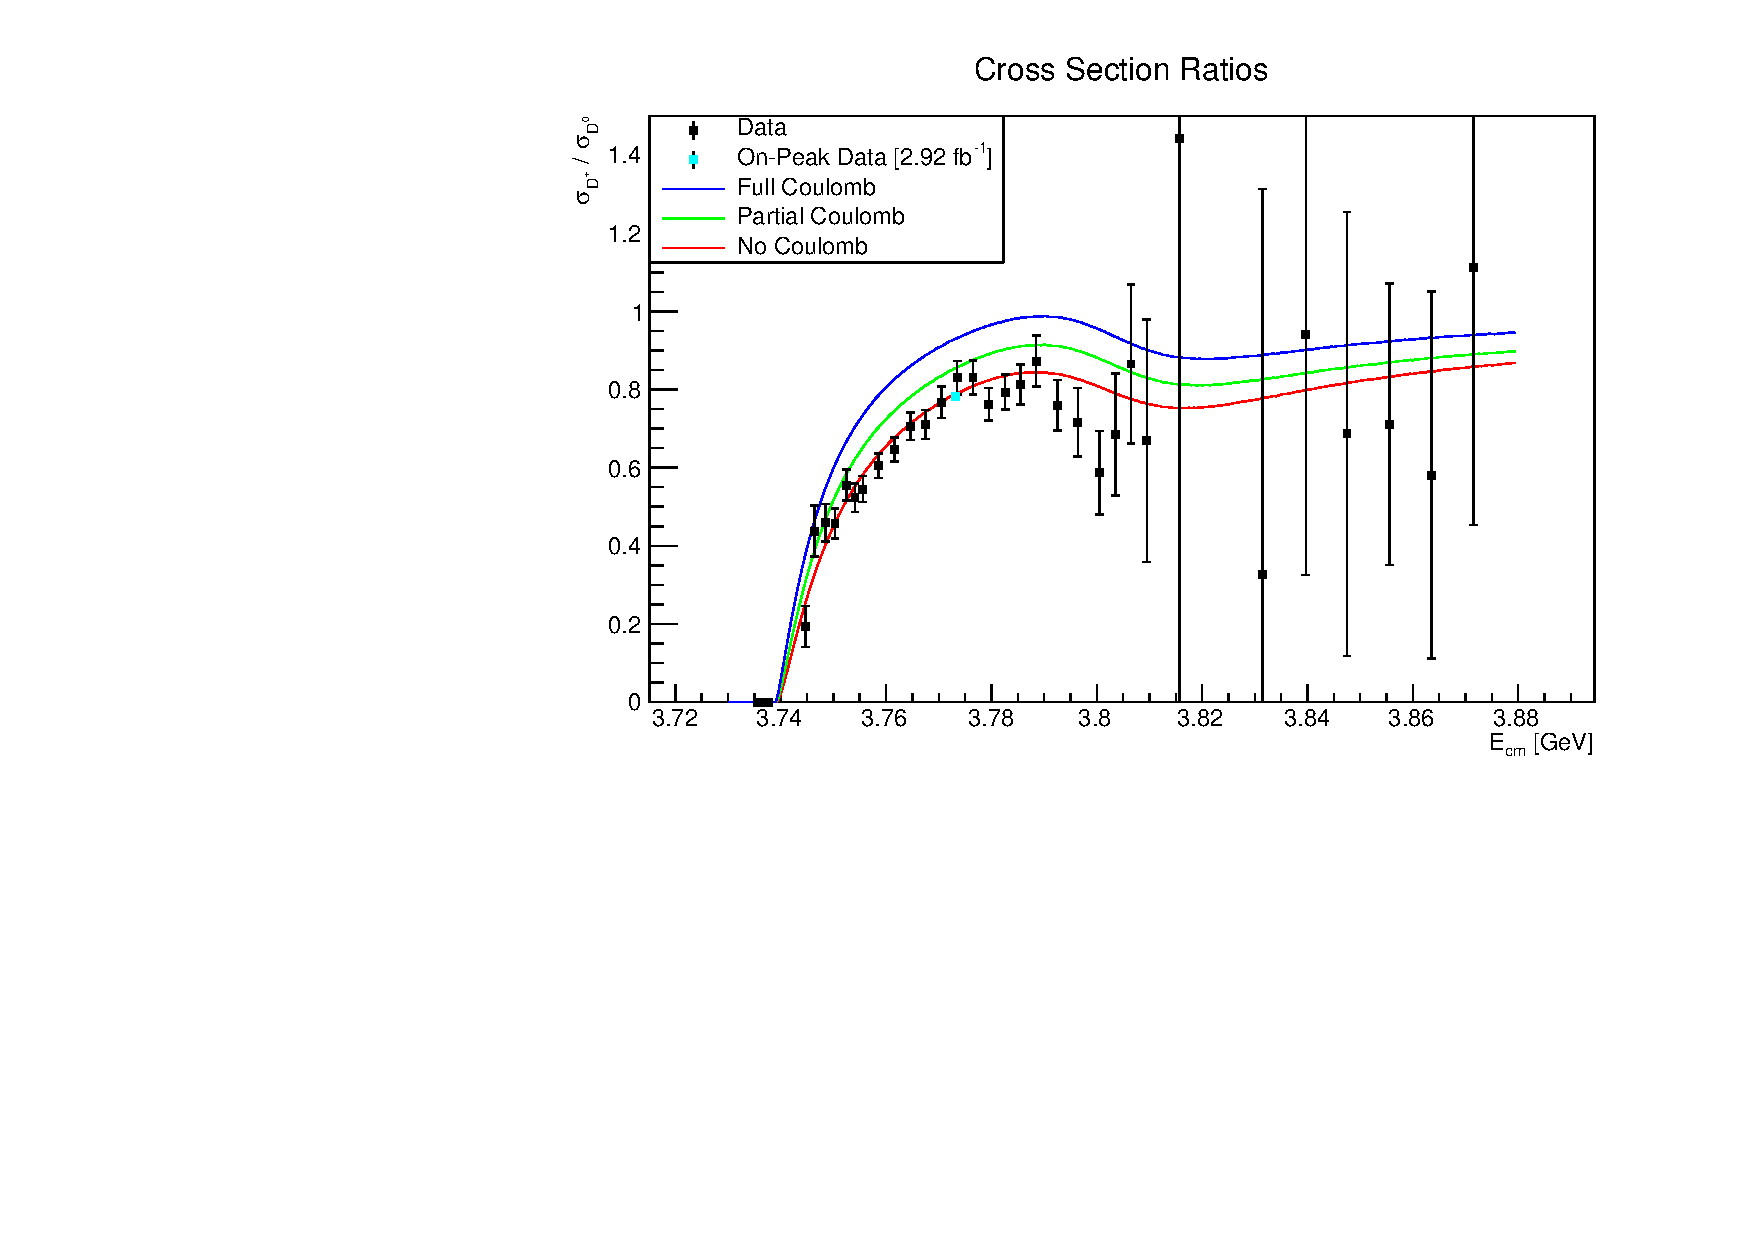
\includegraphics[scale=0.75]{figures/plots/Coulomb_ratio.pdf}
\caption{The ratio of measured $\Dp$ to $\DO$ cross sections.}
{Several levels of Coulomb interactions are examined.}
\label{fig:Coulomb_ratio}
\end{figure}

\pagebreak


\section{Systematic Uncertainties}
\label{sec:systematics}

To assess the systematic uncertainties in our results, we look at a variety of factors.
Many of these affect all BESIII analyses, such as luminosity and tracking.
Others, like the modification to KKMC generation (see \Cref{ssec:monte_carlo}), are specific to this analysis.
Additional analysis-specific systematics are typically due to less well-known parameters, like the radii used to describe the $\psip$ and $\psipp$ (see \Cref{sec:form_factors}).
Each of these contributions, as well as their total, can be found in \Cref{tab:systematics}. 


\subsection{$\psipp$ Parameter Systematic Uncertainties}
\label{ssec:sys_psipp}

Each systematic is obtained by changing a specific assumption, selection criteria, or another analysis feature and re-fitting to the altered cross section distribution using the VDM method.
The uncertainties for each parameter are obtained by taking the difference between this result and the nominal fit (\Cref{fig:vdm_results}).
Generally, each change was done both positively and negatively, and the values used are the largest differences seen between the two changes.
The systematics examined in this analysis are summarized below, where a * denotes potential sources that were found to be negligible.


\subsection*{Luminosity}
\label{ssec:sys_luminosity}

A \SI{1}{\%} change \cite{ref:Ablikim:2013b} was applied to $\lum$ in \Cref{eq:xsec_rc_data}.
As this is an overall scale change, the only variable significantly affected is $\GeepsipptoDD$.


\subsection*{$\pipm / \Kpm$ Tracking}
\label{ssec:sys_Kpi_tracking}

A \SI{1.0}{\%} efficiency change \cite{ref:Rong:2015} was applied for each $\pipm$ or $\Kpm$ in a given decay mode.  
The summed contribution for each mode is applied to $\epsilon_m$ in \Cref{eq:DDbar_eff}.
As this is an overall scale change, the only variable significantly affected is $\GeepsipptoDD$.


\subsection*{$\piO$ Tracking}
\label{ssec:sys_pi0_tracking}

A \SI{2.0}{\%} efficiency change \cite{ref:Ke:2015} was applied for each $\piO$ in a given decay mode.
The summed contribution for each mode is applied to $\epsilon_m$ in \Cref{eq:DDbar_eff}.
As this is an overall scale change, the only variable significantly affected is $\GeepsipptoDD$.


\subsection*{$\Ks$ Tracking}
\label{ssec:sys_Ks_tracking}

A \SI{1.5}{\%} efficiency change \cite{ref:Ma:2014} was applied for each $\Ks$ in a given decay mode.
The summed contribution for each mode is applied to $\epsilon_m$ in \Cref{eq:DDbar_eff}.
As this is an overall scale change, the only variable significantly affected is $\GeepsipptoDD$.


\subsection*{Single Tag Fitting}
\label{ssec:sys_single_tag}

A mode-dependent change \cite{ref:Toth:2014} was applied to $N$ in \Cref{eq:xsec_rc_data}.
Differences from fitting were obtained by Derrick Toth after examining the use of single-Gaussian convolved signal shapes as alternatives to the standard procedure, and are shown in \Cref{tab:sys_single_tag}. 
The changes applied were obtained from the sums of the mode-dependent values averaged over their efficiencies.
As this is an overall scale change, the only variable significantly affected is $\GeepsipptoDD$.


\begin{table}[H]
\centering
\renewcommand\arraystretch{1.0}
\begin{tabular}{l|c||l|c}
\hline
\multicolumn{1}{c|}{Tag Mode} & Difference (\%) & \multicolumn{1}{c|}{Tag Mode} & Difference (\%) \\
\hline
$\DOmodeA$ & 0.27 & $\DpmodeA$ & 0.20 \\
$\DOmodeB$ & 0.10 & $\DpmodeB$ & 0.00 \\
$\DOmodeC$ & 0.47 & $\DpmodeC$ & 0.17 \\
           &      & $\DpmodeD$ & 0.29 \\
           &      & $\DpmodeE$ & 0.17 \\
           &      & $\DpmodeF$ & 0.74 \\
\hline
\multicolumn{2}{c||}{$\DO$ Average: \SI{0.25}{\%}} & \multicolumn{2}{c}{$\Dp$ Average: \SI{0.20}{\%}} \\ [1pt]
\hline
\end{tabular}
\caption{Single-tag fitting differences by mode.}
{The total $\DO$ and $\Dp$ values are averaged over the efficiencies for each mode.}
\label{tab:sys_single_tag}
\end{table}


\subsection*{PDG Branching Fractions}
\label{ssec:sys_pdg}

A mode-dependent change based on the PDG branching fractions (\Cref{tab:DTag_eff}) was applied to $\epsilon_m$ in \Cref{eq:DDbar_eff}.
The branching fraction for each mode was changed by its error. 
As this is an overall scale change, the only variable significantly affected is $\GeepsipptoDD$.

\pagebreak

\subsection*{Meson Radii}
\label{ssec:sys_radii}

The most uncertain parameters used in the analysis are the radii of the mesons $\psip$ and $\psipp$, which enter through the cross section parametrization
We take the same values as used by KEDR, however, each of these is quoted to have an $\sim$25\% uncertainty.
With this, we adjust the two radii values up or down by 25\% over the four possible combinations (both up, both down, and each opposite).
The maximum deviations from the nominal method seen across all four cases are used as the systematic uncertainties.
Due to the high level of uncertainty on these parameters, this effect is one of the largest sources of systematic uncertainty in the analysis.


\subsection*{MC Iteration*}
\label{ssec:sys_kkmc}

In generating MC for this analysis, the $\DDbar$ samples used a modified form of KKMC which generates events based on an input Born level shape for the $\psipp$.
However, as this shape is also the final output of the analysis, only an estimate is available for generation.
To assess the variation from the input shape, we compared the output fit parameters to those used in the generation process.
This process used the Exponential method, and the results are shown in \Cref{tab:KKMC_parameters}.
The numbers listed are from an earlier iteration of the MC that than shown in \Cref{sec:fitting}, but the consistency seen is representative of all iterations.
Very little difference is seen in the primary fit output parameters of the $\psipp$.
These similarities show the fit values converging, even after only a single iteration.
From this, we treat variations due to MC iteration as negligible.

\begin{table}[H]
\centering
\renewcommand\arraystretch{1.0}
\begin{tabular}{l c|r@{ $\pm$ }l r@{ $\pm$ }l|c}
\hline
\multicolumn{2}{c}{Parameter} & \multicolumn{2}{c}{KKMC Input} & \multicolumn{2}{c}{Fit Results} & Difference \\
\hline
$\Mpsipp$       & [\si{\GeV}] &   3.7815 &  0.0003 &   3.7814 &  0.0003 & 0.0001 \\
$\Gpsipp$       & [\si{\MeV}] &  24.887  &  0.686  &  24.839  &  0.681  & 0.048  \\
$\GeepsipptoDD$ & [\si{\eV}]  & 217.55   & 11.18   & 214.65   & 11.10   & 2.90   \\
$\Ppsipp$       &             &   3.6374 &  0.0513 &   3.6375 &  0.0518 & 0.0001 \\
$\FNR$          &             &  21.394  &  1.866  &  20.147  &  1.765  & 0.992  \\
$\aNR$          &             &  -1.6202 &  0.5271 &  -1.5265 &  0.5119 & 0.0937 \\
\hline
\end{tabular} 
\caption{Comparison of input and output fit parameters.}
{The MC generation is done using the Exponential form factor model as an input Born level shape to generate $\DDbar$ events using KKMC.}
\label{tab:KKMC_parameters}
\end{table}


\subsection*{MC ISR Generation*}
\label{ssec:sys_conexc}

To compare to the generation process of KKMC, we also generated alternative MC samples of $\DDbar$ using the ConExc \cite{ref:Ping:2014} ISR generator.
This process used an input Born level shape identical to a previous iteration produced with KKMC.
Each of the background samples used (such as $\qqbar$ and $\tautau$) were the same as in the nominal procedure.
The cross section results using the VDM model are shown in \Cref{tab:ConExc}, and provide $\psipp$ fit parameters that are within the statistical errors of the nominal method.
From this, we treat variations due to the MC ISR generator as negligible.

\begin{table}[H]
\centering
\renewcommand\arraystretch{1.0}
\begin{tabular}{l c|r@{ $\pm$ }l r@{ $\pm$ }l}
\hline
\multicolumn{2}{c}{Parameter} & \multicolumn{2}{c}{ConExc Fit Results} & \multicolumn{2}{c}{KKMC Fit Results} \\
\hline
$\Mpsipp$       & [\si{\GeV}] &   3.7803 &  0.0003 &   3.7804 &  0.0003 \\
$\Gpsipp$       & [\si{\MeV}] &  23.784  &  0.616  &  23.732  &  0.612  \\
$\GeepsipptoDD$ & [\si{\eV}]  & 204.68   & 10.28   & 207.35   & 10.02   \\
$\Ppsipp$       &             &   3.5954 &  0.0559 &   3.5952 &  0.0525 \\
$\Geepsip$      & [\si{\MeV}] &  12.229  &  1.336  &  14.070  &  1.431  \\
$F_0$           &             &  -2.3415 &  0.4898 &  -2.0768 &  0.4924 \\
\hline
\end{tabular} 
\caption{Comparison of output fit parameters between ISR generators.}
{The MC generation is done using both the ConExc and KKMC generators and the final VDM fit results are shown.
The values shown are from an earlier iteration than the final results, but the output from each method remains very similar.}
\label{tab:ConExc}
\end{table}



% \begin{figure}[H]
% \centering
% 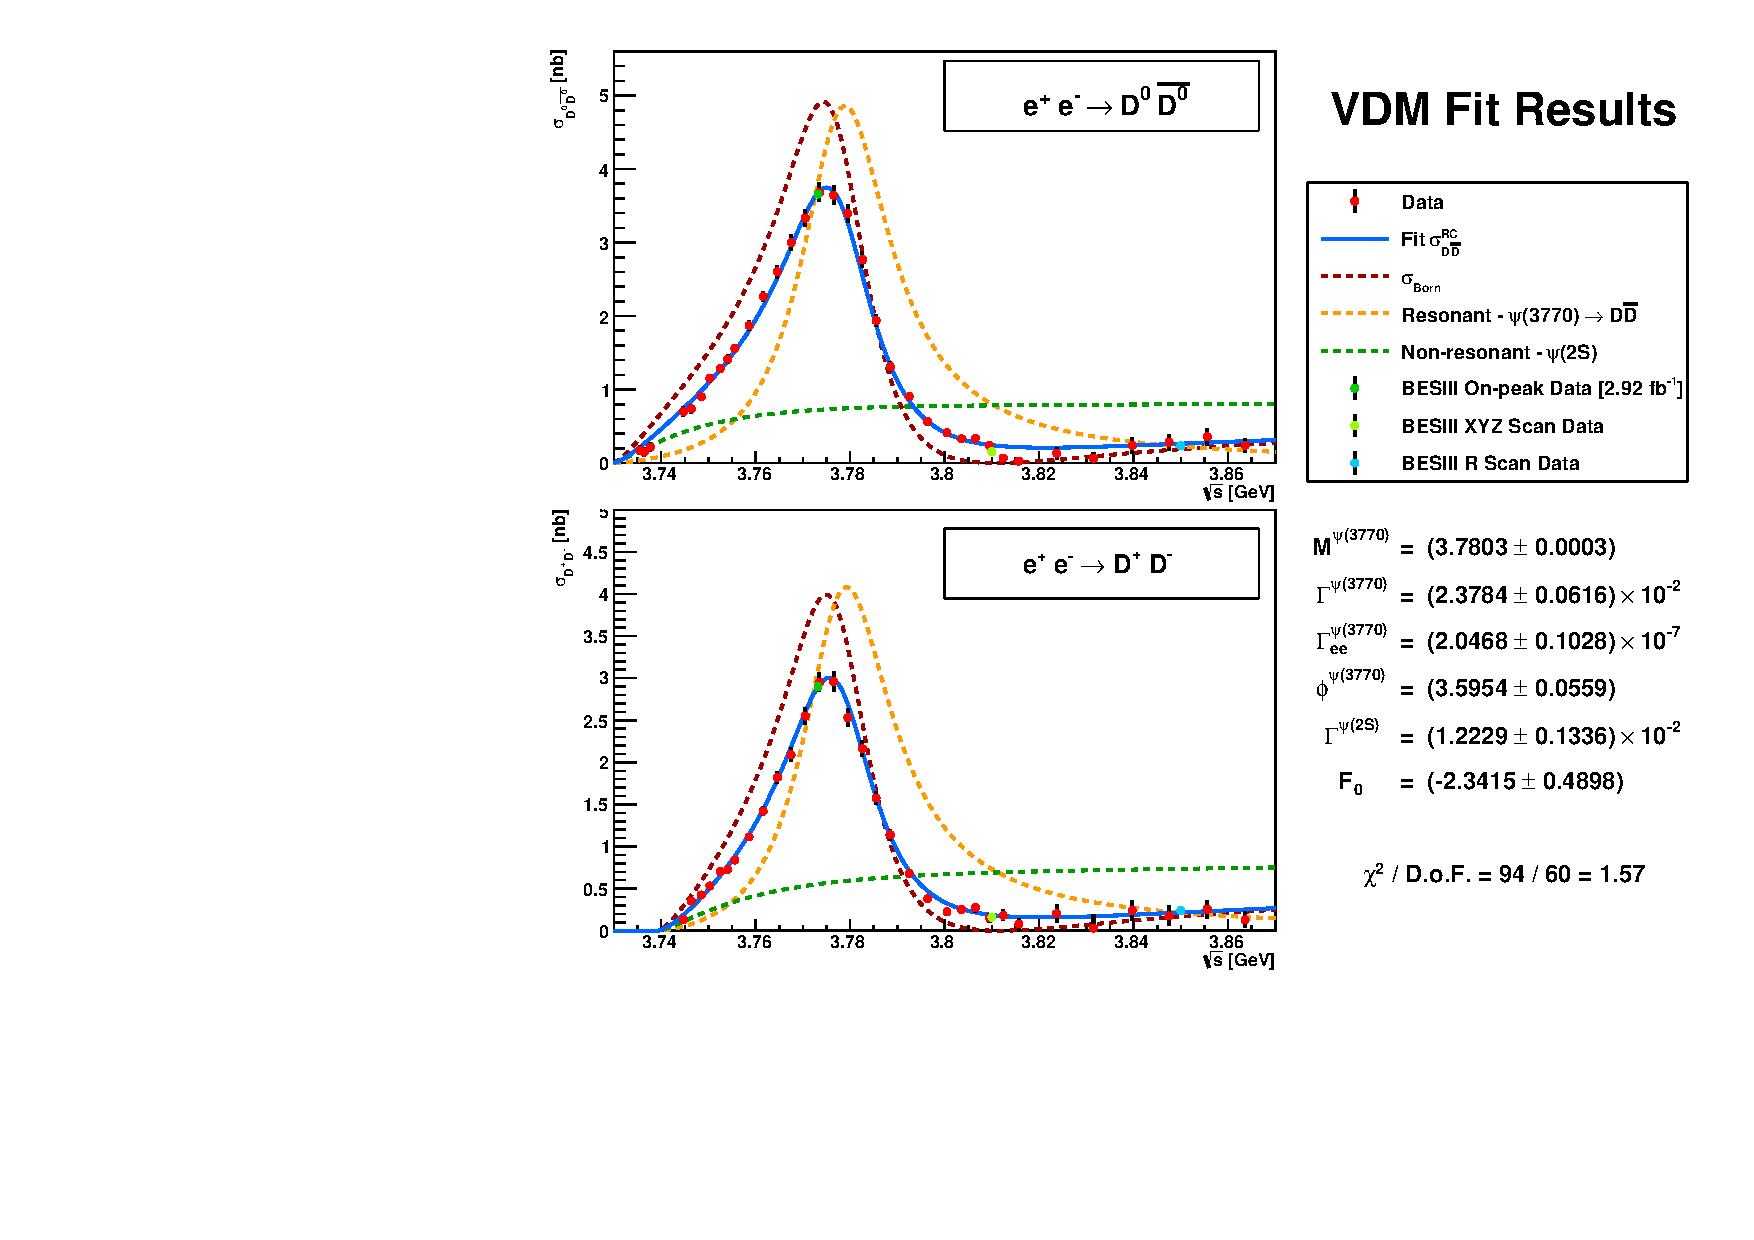
\includegraphics[scale=0.75]{figures/plots/lineshape_vdm_ConExc.pdf}
% \caption{The Vector Dominance Model fit results using ConExc.}
% {The results for $\DO$ are shown on the top and the results for $\Dp$ are shown on the bottom. The underlying MC shapes for the  $\DDbar$ components were generated with an alternative generator to compare to KKMC.}
% \label{fig:ConExc}
% \end{figure}

\pagebreak

\subsection*{Intermediate Resonances*}
\label{ssec:sys_intermediate_resonances}

In looking at the mode $\DpmodeA$, we also analyzed the contribution of intermediate resonances to the $\pip\pim$ system, like the $\rho^0$.
Using the \SI{2.93}{\invfb} data sample of $\psipp$ events at $\Ecm = \SI{3.773}{\GeV}$, we split the signal region of this mode based on \SI{1.0}{\GeV^2} cuts for each of the invariant masses of $K \pi$ and $\pi \pi$.
These cuts were chosen to separate the sample into distinctly different regions, as can be seen in \Cref{fig:Kpipi_mass}.
Fitting the signal distributions for each of these subsamples, we found no statistically significant deviations in the measured yields, and treat this contribution as negligible.
% From this, we treat variations due to intermediate resonances as negligible.

\begin{figure}[H]
\centering
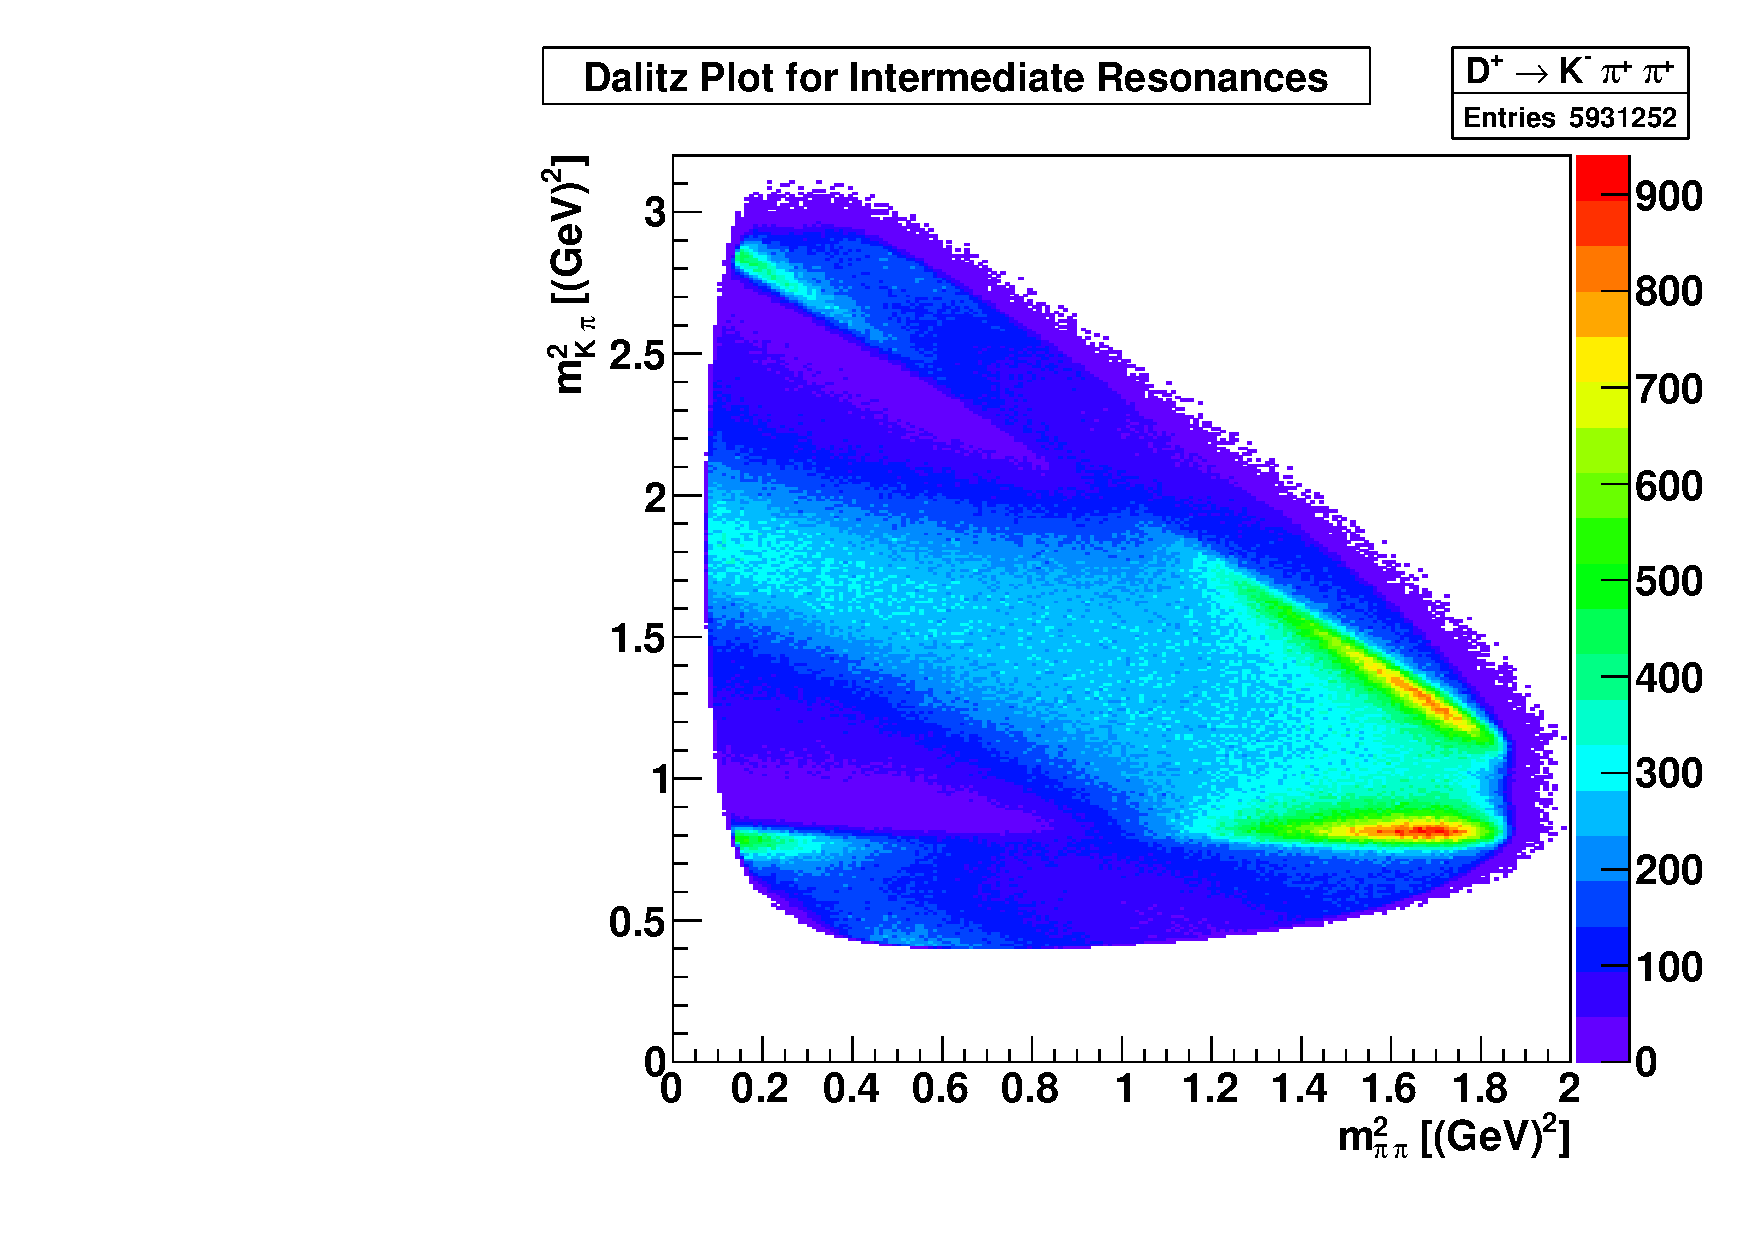
\includegraphics[scale=0.5]{figures/plots/Kpi_vs_pipi_Ecm.pdf}
\caption{The $K \pi$ vs. $\pi \pi$ invariant masses for the mode $\DpmodeA$.}
{The on-peak $\psipp$ data was used due to its significantly higher statistics.}
\label{fig:Kpipi_mass}
\end{figure}

\pagebreak

\subsection*{Total Systematic Uncertainties}
\label{ssec:sys_total}

Each of the systematic uncertainty sources considered are assumed to be independent, meaning they are combined in quadrature for the total value.
The results are shown in \Cref{tab:systematics} along with a comparison to the statistical error.
Because of the large uncertainty on the meson radii, our measurements are systematics limited, even given the relatively small data sample used.

\begin{table}[H]
\centering
\renewcommand\arraystretch{1.0}
\begin{tabular}{c|cccc}
\hline 
Systematic & $\Mpsipp$ [\%] & $\Gpsipp$ [\%] & $\GeepsipptoDD$ [\%] & $\Ppsipp$ [\%] \\
\hline 
Luminosity              & 0.000 & 0.004 & 1.005 & 0.014 \\
$\Kpm / \pipm$ Tracking & 0.000 & 0.008 & 2.646 & 0.033 \\
$\piO$ Tracking         & 0.000 & 0.012 & 0.746 & 0.028 \\
$\Ks$ Tracking          & 0.000 & 0.004 & 0.260 & 0.019 \\ 
Single Tag Fits         & 0.000 & 0.012 & 0.213 & 0.008 \\
PDG Errors              & 0.000 & 0.017 & 2.840 & 0.036 \\
Meson Radii             & 0.016 & 2.411 & 3.512 & 1.477 \\
\hline
Total [\%]                      & 0.016 & 2.411 & 5.389 & 1.479 \\
Relative Stat. Error [$\sigma$] & 3.000 & 1.088 & 1.342 & 1.229 \\
\hline
\end{tabular} 
\caption{Systematic uncertainties relative to the measured parameters of the $\psipp$.}
\label{tab:systematics}
\end{table}


\subsection*{Non-Resonant Form Factor}
\label{ssec:sys_form_factor}

In addition to the systematics described above, there is a significant source of uncertainty coming from the non-resonant form factor used.
Both models examined, Exponential and VDM, provided quality fit results for the cross section shapes.
From this, we conservatively assign an uncertainty equal to the differences in fit parameters provided by these two methods, as shown in \Cref{tab:sys_form_factor}.
Following the example of KEDR, we treat this as a model-dependent uncertainty separate from the other systematics.

\begin{table}[H]
\centering
\renewcommand\arraystretch{1.0}
\begin{tabular}{c|cccc}
\hline 
Form Factor & $\Mpsipp$ [\si{\GeV}] & $\Gpsipp$ [\si{\MeV}] & $\GeepsipptoDD$ [\si{\eV}] & $\Ppsipp$ [\si{\degree}] \\
\hline 
VDM & 3.7821 & 26.004 & 233.13 & 214.60 \\
VDM & 3.7808 & 24.098 & 215.83 & 207.12 \\
\hline
Difference & 0.0013 & 1.906 & 17.30 & 7.48 \\
\hline
\end{tabular} 
\caption{Parameter differences based on the choice of form factor.}
{These are treated as model-dependent errors, not as part of the total systematics.}
\label{tab:sys_form_factor}
\end{table}



\subsection{Cross Section Systematic Uncertainties}
\label{ssec:sys_cross_section}

In addition to the statistical uncertainties provided in \Cref{tab:xsec_rc_data}, we also provide systematic uncertainties on the cross section measurements.
These are calculated from the systematic shifts ($\Delta S$) which affect \Cref{eq:xsec_rc_data}: Luminosity, $\Kpm / \pipm$ Tracking, $\piO$ Tracking, $\Ks$ Tracking, and Single Tag Fits.
For the luminosity, this is the same as the $\pm1\%$ shift used previously.
The others are calculated by weighting the efficiency over decay modes:
\beq
\Delta S = \frac{ \sum\limits_m \epsilon_m \Delta S_m }{ \sum\limits_m \epsilon_m }
\eeq
The value of $\Delta S_m$ for $\Kpm / \pipm$ Tracking is 1.0\% per $\Kpm$ or $\pipm$, and is defined similarly for the other systematics using the previously listed values.
The calculated shifts are listed in \Cref{tab:sys_shifts}, and the resulting cross section values are listed in \Cref{tab:xsec_rc_data_sys}.


\begin{table}[H]
\centering
\renewcommand\arraystretch{1.0}
\begin{tabular}{c|cc}
\hline 
Systematic & $\Delta S$ ($\DO$) [\%]  & $\Delta S$ ($\Dp$) [\%] \\
\hline 
Luminosity              & 1.00 & 1.00 \\
$\Kpm / \pipm$ Tracking & 2.58 & 2.59 \\
$\piO$ Tracking         & 0.94 & 0.63 \\
$\Ks$ Tracking          & 0.00 & 0.42 \\ 
Single Tag Fits         & 0.25 & 0.20 \\
PDG Error               & 0.31 & 0.18 \\
\hline
Total                   & 2.95 & 2.89 \\
\hline
\end{tabular} 
\caption{Systematics shifts affecting the cross section measurements.}
    {The total shifts are used to calculate the systematic uncertainties of the $\DO$ and $\Dp$ cross sections.}
\label{tab:sys_shifts}
\end{table}


\begin{table}[H]
\centering
\renewcommand\arraystretch{1.0}
\begin{tabular}{c|c@{$\; \pm \;$}c@{$\; \pm \;$}c c@{$\; \pm \;$}c@{$\; \pm \;$}c}
\hline 
$E_{\text{mid}}$ [GeV] & \multicolumn{3}{c}{$\sigma^{RC}_{\DO \aDO}$ [nb]} & \multicolumn{3}{c}{$\sigma^{RC}_{\Dp \Dm}$ [nb]} \\
\hline

3.7342 & 0.164 & 0.046 & 0.005 & \multicolumn{2}{c}{-} \\
3.7368 & 0.218 & 0.068 & 0.006 & \multicolumn{2}{c}{-} \\
3.7447 & 0.765 & 0.070 & 0.023 & 0.150 & 0.038 & 0.004 \\
3.7483 & 0.838 & 0.064 & 0.025 & 0.360 & 0.048 & 0.010 \\
3.7501 & 0.968 & 0.053 & 0.029 & 0.439 & 0.040 & 0.013 \\
3.7517 & 1.237 & 0.052 & 0.036 & 0.574 & 0.040 & 0.017 \\
3.7534 & 1.377 & 0.051 & 0.041 & 0.748 & 0.042 & 0.022 \\
3.7556 & 1.566 & 0.055 & 0.046 & 0.797 & 0.045 & 0.023 \\
3.7562 & 1.629 & 0.051 & 0.048 & 0.914 & 0.042 & 0.026 \\
3.7592 & 1.948 & 0.052 & 0.057 & 1.192 & 0.045 & 0.034 \\
3.7624 & 2.385 & 0.058 & 0.070 & 1.534 & 0.051 & 0.044 \\
3.7650 & 2.715 & 0.071 & 0.080 & 1.882 & 0.066 & 0.054 \\
3.7676 & 3.102 & 0.087 & 0.092 & 2.200 & 0.081 & 0.064 \\
3.7713 & 3.406 & 0.101 & 0.100 & 2.634 & 0.098 & 0.076 \\
3.7742 & 3.714 & 0.111 & 0.110 & 3.067 & 0.111 & 0.089 \\
3.7775 & 3.692 & 0.111 & 0.109 & 3.078 & 0.111 & 0.089 \\
3.7802 & 3.444 & 0.104 & 0.102 & 2.599 & 0.100 & 0.075 \\
3.7829 & 2.791 & 0.090 & 0.082 & 2.206 & 0.088 & 0.064 \\
3.7869 & 1.995 & 0.072 & 0.059 & 1.627 & 0.073 & 0.047 \\
3.7891 & 1.361 & 0.058 & 0.040 & 1.178 & 0.062 & 0.034 \\
3.7926 & 0.920 & 0.045 & 0.027 & 0.680 & 0.045 & 0.020 \\
3.7970 & 0.562 & 0.037 & 0.017 & 0.414 & 0.039 & 0.012 \\
3.8003 & 0.424 & 0.035 & 0.013 & 0.241 & 0.037 & 0.007 \\
3.8024 & 0.325 & 0.038 & 0.010 & 0.236 & 0.043 & 0.007 \\
3.8070 & 0.352 & 0.050 & 0.010 & 0.289 & 0.051 & 0.008 \\
3.8093 & 0.233 & 0.050 & 0.007 & 0.132 & 0.055 & 0.004 \\
3.8135 & 0.060 & 0.049 & 0.002 & 0.153 & 0.066 & 0.004 \\
3.8153 & 0.056 & 0.051 & 0.002 & 0.089 & 0.063 & 0.003 \\
3.8229 & 0.140 & 0.083 & 0.004 & 0.197 & 0.107 & 0.006 \\
3.8320 & 0.069 & 0.086 & 0.002 & 0.046 & 0.099 & 0.001 \\
3.8390 & 0.237 & 0.105 & 0.007 & 0.254 & 0.124 & 0.007 \\
3.8494 & 0.186 & 0.104 & 0.005 & 0.186 & 0.118 & 0.005 \\
3.8555 & 0.337 & 0.111 & 0.010 & 0.273 & 0.104 & 0.008 \\
3.8632 & 0.340 & 0.127 & 0.010 & 0.099 & 0.091 & 0.003 \\
\hline
\end{tabular} 
\caption{Measurements of the $\DO$ / $\Dp$ cross sections.}
{The first errors are statistical and the second are systematic.}
\label{tab:xsec_rc_data_sys}
\end{table}


\section{Results}
\label{sec:results}

After incorporating the systematic and model uncertainties, the total results for the main $\psipp$ parameters are shown in \Cref{tab:results}.
The results shown are from the VDM model, as we treat this as the nominal results.
The Exponential model is used as a measure of uncertainty, however, the quality of fits found by this approach means it cannot be excluded as a viable option.

\begin{table}[H]
\centering
\renewcommand\arraystretch{1.0}
\begin{tabular}{C{2.25cm} l c}
\hline 
$\Mpsipp$       & $    3780.8 \pm     0.2   \pm    0.6   \pm   1.3$ & $[\si{\MeV}]$   \\
$\Gpsipp$       & $\PP 24.1   \pm     0.5   \pm    0.6   \pm   1.9$ & $[\si{\MeV}]$   \\
$\GeepsipptoDD$ & $\PP 216 \; \pm \pp  9 \; \pm    11 \; \pm    17$ & $[\si{\eV}]$    \\
$\Ppsipp$       & $\PP 207 \; \pm \pp  3 \; \pm \pp 3 \; \pm \pp 7$ & $[\si{^\circ}]$ \\
\hline
\end{tabular} 
\caption{Final results for the $\psipp$ parameters.}
{The first error listed is statistical, the second is systematic, and the third is from the form factor model.}
\label{tab:results}
\end{table}


Additionally, since this analysis is based on an approach developed by the KEDR collaboration, a comparison to their results is also shown in \cref{tab:fit_results}.  
For their measurement of $\Geepsipp$, two solutions were found with very close $\chi^2$ values, so both are quoted in their final results.
With the larger statistics available at BESIII, no alternate solution was found during searches over the parameter space.
It is clear the VDM results are well in line with the parameters found by the KEDR collaboration, but with significantly smaller statistical errors.
Each of these measurements are also highly discrepant with the current PDG world averages.

\begin{table}[H]
\centering
\renewcommand\arraystretch{1.0}
\begin{tabular}{C{3cm} L{3cm} L{3cm} L{3cm}}
\hline
Method & $\Mpsipp$ [MeV] & $\Gpsipp$ [MeV] & $\GeepsipptoDD$ [eV] \\
\hline
Exponential & $3782.1 \pm 0.3 \pm 0.6$ & $26.0 \pm 0.6 \pm 0.7$ & $233 \pm 10 \pm 13$ \\
VDM         & $3780.8 \pm 0.2 \pm 0.6$ & $24.1 \pm 0.6 \pm 0.6$ & $216 \pm  9 \pm 12$ \\
KEDR        & $3779.2^{+1.8 +0.5 +0.3}_{-1.7 -0.7 -0.3}$ & $24.9^{+4.6 + 0.5 +0.2}_{-4.0 -0.6 -0.9}$ & $154^{+79 +17 +13}_{-58 -9\pp -25}$, $414^{+72 +24 +90}_{-80 -26 -10}$ \\
PDG         & $3773.15 \pm 0.33$     & $27.2 \pm 0.9$       & $[262 \pm 18] \times ~\BDD$ \\
\hline
\end{tabular}
\caption{Fit results compared to the KEDR results and the PDG.}
{The first errors listed are statistical, while the second are systematic.  In the case of KEDR, the third error is from the model. }
\label{tab:fit_results}
\end{table}

\pagebreak

We can also compare our results to the cross section values found in the previous analysis of BESIII's on-peak $\psipp$ data sample of \SI{2.93}{\invfb} by Derrick Toth \cite{ref:Toth:2014}.
The values displayed on \Cref{fig:exp_results,fig:vdm_results} are his double-tag (DT) values.
Each of these cross sections are shown in \Cref{tab:Derrick_xsec}.
Further analysis to better understand the differences seen is still in progress, however both methods used in this analysis are within ${\sim}1\sigma$ of the high statistics method.

\begin{table}[H]
\centering
\renewcommand\arraystretch{1.2}
\begin{tabular}{C{3cm} L{3.5cm} L{3.5cm}}
\hline
Model & \multicolumn{1}{c}{$\sigma_{\DO \aDO}$ [nb]} & \multicolumn{1}{c}{$\sigma_{\Dp \Dm}$ [nb]} \\
\hline
Derrick (DT) & $3.615 \pm 0.010 \pm 0.035$ & $2.830 \pm 0.011 \pm 0.026$ \\
Exponential  & $3.662 \pm 0.131 \pm 0.108$ & $2.947 \pm 0.118 \pm 0.085$ \\
VDM          & $3.748 \pm 0.131 \pm 0.111$ & $2.951 \pm 0.118 \pm 0.085$ \\
\hline
\end{tabular}
\caption{Comparison of cross section calculations at $\Ecm = \SI{3.7732}{\GeV}$}
    {The values measured previously used a \SI{2.93}{\invfb} data sample of $\psipp$ events to reconstruct double-tag (DT) decays.  The first errors listed are statistical, while the second is systematic.}
\label{tab:Derrick_xsec}
\end{table}


